% !TeX program = xelatex
% !TeX encoding = UTF-8

% ================================ CLASS OPTIONS ====================================
% Default setup (recommended):
\documentclass[a4paper,12pt,oneside]{CityUHKThesis}
%
% Alternative setup:
% twoside: automatically insert a blank verso page
% fancychap: use fancy chapter title style (Lenny)
% \documentclass[a4paper,12pt,twoside,fancychap]{CityUHKThesis}

% ================================ LAYOUT & SPACING =================================
\setlength{\parskip}{.5em}
\raggedbottom

% ================================ PACKAGE LOADING ==================================
% Lists and formatting
\usepackage{enumitem}
\setlist[enumerate,itemize,description]{topsep=0em}

% Tables and figures
\RequirePackage[labelsep=period,tableposition=top,labelfont=bf,textformat=period]{caption}
\usepackage{subfigure}
\usepackage{booktabs}
\usepackage{multirow}
\usepackage[flushleft]{threeparttable}
\newcommand{\mtnote}[1]{\textsuperscript{\TPTtagStyle{#1}}}

% ================================ BIBLIOGRAPHY SETUP ===============================
\usepackage[
  style=ACM-Reference-Format,
  citestyle=numeric-comp,
  backend=biber,
  sortcites=true,
  backref=true,
  doi=false,
  isbn=false,
  url=true,
  eprint=false,
  maxbibnames=99,
  maxcitenames=2,
  giveninits=true
]{biblatex}

\appto{\bibsetup}{\sloppy}
\addbibresource{References/references.bib}

% Optimize citation formatting
\renewcommand*{\nameyeardelim}{\addcomma\space}
\DeclareFieldFormat{postnote}{#1}
\DeclareFieldFormat{multipostnote}{#1}

% ================================ CITATION HELPERS =================================
\usepackage{breakcites}
\newcommand\spacecite{\penalty700\ \cite}

% ================================ DOCUMENT STRUCTURE ===============================
\setcounter{secnumdepth}{3}
\setcounter{tocdepth}{2}

% ================================ TYPOGRAPHY =======================================
\usepackage{microtype}
\usepackage{underscore}

% Conditional content for development
\usepackage{lipsum} % Remove in final version

% ================================ MATH & THEOREMS ==================================
\usepackage{amsthm}
\theoremstyle{definition}
\newtheorem{definition}{Definition}[chapter]
\newtheorem{example}[definition]{Example}
\newtheorem{remark}[definition]{Remark}

\theoremstyle{plain}
\newtheorem{theorem}[definition]{Theorem}
\newtheorem{lemma}[definition]{Lemma}
\newtheorem{corollary}[definition]{Corollary}
\newtheorem{proposition}[definition]{Proposition}

% ================================ ALGORITHMS =======================================
\usepackage{algorithm}
\usepackage{algorithmicx}
\usepackage{algpseudocode}

% ================================ DEVELOPMENT HELPERS ==============================
\newcommand{\fixme}[1]{\textcolor{red}{#1}}
% \newcommand{\todo}[1]{\textcolor{blue}{\textbf{TODO:} #1}} % Uncomment if needed

% ================================ XETEX SETTINGS ===================================
\XeTeXgenerateactualtext=1



% ================================ COMPILATION OPTIMIZATIONS ========================
\hbadness=999999
\hfuzz=9999pt

% ================================ GRAPHICS PATH ====================================
\graphicspath{
  {FrontMatter/figures/}
  {Chapters/paperone/figures/}
  {Chapters/papertwo/figures/}
  {Chapters/paperthree/figures/}
}

% ================================ DOCUMENT METADATA ================================
\title{Design, Modeling, and Control of a Water-Skipping Micro Aerial Vehicle}
\titlezh{水面弹跳微型无人机的设计、建模与控制研究}

\author{Wang Fang Zheng}
\authorzh{王方正}

\university{City University of Hong Kong}
\universityzh{香港城市大學}
\universityabbr{CityU}
% For joint PhD programme, uncomment the following line
%\partneruniversity{University of Science and Technology of China}

\dept{Department of Public Policy}
\deptzh{公共政策學系}

\degreetitle{Mater of Philosophy} % Master/Doctor of Philosophy as appropriate
\degreetitlezh{哲學硕士學位} % 哲學碩士/博士學位 as appropriate
\degreetitleabbr{Mphil} % MPhil or PhD as appropriate

\degreedate{June 2026} % Available in the AIMS after oral examination
\degreedatezh{二零二六年六月}

\subject{Ph.D. Thesis}
\keywords{{keyword one}; {keyword two}; {keyword three}; {keyword four}}

% ================================ DOCUMENT CONTENT ================================
\begin{document}

\frontmatter

\maketitle
\cleardoublepageempty

\include{FrontMatter/dedication} % Optional
\begin{abstract}

This thesis presents a micro aerial vehicle that travels across water in a
sequence of hops, driven by hydrofoils that rotate with the airframe. Inspired
by stone-skipping, the vehicle descends onto a water surface with its lift
rotors switched off; the spinning hydrofoils submerge briefly, generate a large
upward impulse, and eject the vehicle back into the air, where it recovers
altitude under closed-loop control and repeats the cycle. Because water is
nearly three orders of magnitude denser than air, the same foils that produce a
negligible force in flight produce a large one on contact, so they cost the
vehicle little while airborne yet supply the whole of the impulse that returns
it to the air.

A quasi-steady blade-element model of the submersion phase is developed, giving
the vertical thrust and the resisting torque generated by a foil as it sweeps
through the water, and coupling them to the vertical and rotational motion of
the vehicle. Simulation across the design space identifies the entry velocity
and the foil inclination as the quantities that govern the hop, shows that the
radial extent of the foil is nearly inert once large enough, and exposes the
central tension of the manoeuvre: the rotation that generates the ejecting
force is itself consumed by the water.

The vehicle built to test this is a $90\;\mathrm{g}$ four-rotor airframe that
spins continuously about its vertical axis. Two rotors are mounted
tangentially and drive the rotation directly at a commanded thrust setpoint,
while two remain vertical and provide lift and attitude authority; because the
yaw drive is decoupled from the lift channel, the spin rate becomes a design
parameter rather than an equilibrium the airframe settles into, and the
rotation persists when the lift command is removed entirely. Flight control
for the resulting fast-rotating vehicle is formulated on its gyroscopic reduced
attitude dynamics, together with an online estimator that separates the
spin-synchronous measurement artefact from the attitude estimate.

Flight experiments in a motion-capture environment demonstrate the full cycle.
The descent is flown with the lift rotors commanded to zero and is arrested
with them still off, so the reversal is the work of the hydrofoils alone;
across eight contacts the vehicle enters the water at $-1.53$ to
$-1.85\;\mathrm{m\,s^{-1}}$ and leaves it climbing, recovering on average
$60\%$ of its entry speed. Consecutive hops are demonstrated with the vehicle
returning to within $8\;\mathrm{mm}$ of its previous release height, showing
that the cycle closes rather than that a single impact can be survived. The
vehicle remained controllable at spin rates approaching
$10{,}000^{\circ}\,\mathrm{s^{-1}}$, with no upper limit encountered.

This work establishes water-skipping as a usable mode of locomotion for small
aerial robots, and provides the model, the airframe, and the control needed to
pursue it further.

\end{abstract}

% TODO(frontmatter): panel membership. The supervisor is filled in; the
% remaining names are still the template's placeholders (SMITH John, ZHANG
% San, DOE John, LI Si, WANG Wu) and MUST be replaced with the real panel
% and examiners before submission. This page is completed only for the
% final version, after the oral examination.

\begin{panel}

\begin{tabular}{p{50mm}p{70mm}}
Surname: & WANG\tabularnewline
First Name: & Fang Zheng\tabularnewline
Degree: & Master of Philosophy\tabularnewline
College/Department: & Department of Mechanical Engineering
\end{tabular}

\vspace{2em}

The Qualifying Panel of the above student is composed of:

\vspace{1em}

\begin{tabular}{p{50mm}p{90mm}}
\textit{Supervisor(s)} & \tabularnewline
Prof. CHIRARATTANANON Pakpong 	 & Department of Mechanical Engineering\tabularnewline
 & City University of Hong Kong\\[1em]\tabularnewline

 
\textit{Qualifying Panel Member(s)} & \tabularnewline
Prof. SMITH John 	 & Department of Mechanical Engineering\tabularnewline
 & City University of Hong Kong\\[.2em]\tabularnewline

Prof. ZHANG San 	 & Department of Mechanical Engineering\tabularnewline
 & City University of Hong Kong\\[.2em]\tabularnewline
\end{tabular}

\vspace{2em}

This thesis has been examined and approved by the following examiners:
\vspace{1em}

\begin{tabular}{p{50mm}p{90mm}}
Prof. DOE John 	 & Department of Mechanical Engineering\tabularnewline
 & City University of Hong Kong\\[.2em]\tabularnewline

Prof. SMITH John 	 & Department of Mechanical Engineering\tabularnewline
 & City University of Hong Kong\\[.2em]\tabularnewline

Prof. LI Si  & Department of Mechanical Engineering\tabularnewline
 & City University of Hong Kong\\[.2em]\tabularnewline

Prof. WANG Wu  & College of Electrical Engineering and Computer Science\tabularnewline
 & Institute of Information Science (IIS), Academia Sinica \\[.2em]\tabularnewline
\end{tabular}

\end{panel}
 % Final version only
% TODO(frontmatter): this is yours to write. The structure below is the
% conventional one; replace each bracketed item. Funding sources in
% particular must be named accurately, and collaborators credited by name.

\begin{acknowledgements}

I would like to thank my supervisor, Prof.\ Pakpong Chirarattananon, for his
guidance throughout this work.

% TODO: panel members, by name.
I thank the members of my qualifying panel for their feedback on this research.

% TODO: lab colleagues who contributed. Name them individually, and say what
% each contributed rather than thanking them as a group.
I thank my colleagues in the lab for their help with the flight experiments
and for many useful discussions.

% TODO: funding. Name the grant and the awarding body exactly.
I gratefully acknowledge the financial support that made this research
possible.

Finally, I thank my family and friends for their support throughout.

\end{acknowledgements}
 % Optional

\tableofcontents
\listoffigures
\listoftables

\mainmatter

\chapter{Introduction}
\label{chapter:introduction}

\section{Background and Motivation}
\label{sec:background_motivation}

Micro aerial vehicles (MAVs) have become capable platforms for environmental
monitoring, search and rescue, and inspection, yet the overwhelming majority
operate exclusively in the air.  Many of the environments where small robots
are most useful (rivers, lakes, flooded terrain, and coastal zones) are
dominated by water, and a vehicle confined to flight must expend continuous
power to remain aloft above them.  Extending an MAV's mobility to include the
water surface would broaden its operational envelope to tasks such as water
sampling, surface skimming, and persistent monitoring of aquatic environments,
while allowing the vehicle to rest on or interact with the surface between
flight phases~\cite{floreano2015science,siddall2014launching}.

The central difficulty is not resting on water but leaving it again.  For a
small, weight- and power-constrained vehicle, repeatedly taking off from the
water surface is energetically demanding: overcoming surface adhesion and
accelerating from rest into flight typically requires either oversized thrust
or dedicated launch mechanisms that add mass and complexity.  Vehicles that
leave the water repeatedly do exist, but each departure is a discrete launch
event paid for in full, releasing a store of energy in a single burst: a
water-reactive fuel~\cite{zufferey2019consecutive}, a gas-powered
launcher~\cite{siddall2014launching}, or the combustion of gas generated by
electrolysis~\cite{chen2017biologically}.  The water contact itself contributes
nothing to the departure, so the full cost of leaving is paid again at every
transition, and the number of transitions a vehicle can make is set by the
energy it carries rather than by anything it recovers.

A different possibility is suggested by stone-skipping.  A flat stone thrown
at a shallow angle skips across water because, during each brief contact, the
water produces a large transient hydrodynamic reaction that redirects the
stone upward before it can sink; the contact is short, the energy lost per
bounce is small, and the stone traverses the surface in a sequence of low-cost
hops~\cite{bocquet2003physics,clanet2004secrets}.
This thesis adapts that principle to a powered vehicle: rather than hovering
above the water or floating on it, the vehicle hops across the surface, and the
upward impulse that returns it to the air is supplied by the water during a
brief hydrofoil contact rather than by a launch mechanism carried for the
purpose.  The mechanism that makes this possible is described in
Section~\ref{sec:water_skipping_mechanism}.

\section{Water-Skipping Mechanism}
\label{sec:water_skipping_mechanism}

The vehicle is a four-rotor airframe that rotates continuously about its
vertical axis during flight.  Two of its rotors are mounted horizontally,
tangential to the frame, and drive this rotation directly; the remaining two
are mounted vertically and provide lift and attitude authority, their
aerodynamic reaction torque adding to the rotation rather than cancelling it.
Because the tangential rotors are commanded independently of the lift channel,
the spin rate is a quantity the vehicle sets rather than one it settles into.
Extending from each of the four motor mounts is a leg that drops below the
airframe and then turns outward into a hydrofoil, so that the four hydrofoils
rotate rigidly with the body; as the vehicle spins, each sweeps through a
circular path at a tangential speed set by the spin rate and its radius from
the centre.

A single hop proceeds in the four stages of
Figure~\ref{fig:hop_cycle}.  The vehicle first climbs and then enters a brief
free-fall, descending toward a still water surface.  At contact
the spinning hydrofoils slice into the water, and the combination of their
tangential sweep speed and their inclined attack angle generates a large
hydrodynamic lift.  Because the foils sweep continuously, the submersion needs
to last only about a tenth of a second: the resulting vertical impulse arrests
the descent and ejects the vehicle back into the air, where it recovers
altitude and repeats the cycle.

The mechanism depends on the contrast between the two media the hydrofoils move
through.  Water is nearly three orders of magnitude denser than air, so the
same hydrofoil, sweeping at the same speed, produces a far larger force during
its brief submersion than it does while spinning in air.  The foils therefore
impose almost no penalty on flight, generating negligible lift as the vehicle
hovers and spins, yet deliver a large upward impulse the instant they touch
water.

That impulse is not free, and it is worth being precise about what is recovered
and what is spent.  The reversal is produced by the sweep of the foils rather
than by any elasticity of the surface, and the sweep is braked as it does the
work: roughly $60\%$ of the spin is surrendered over a single contact.  What
the vehicle receives in exchange is measured in
Chapter~\ref{chapter:paperthree}, where it leaves the water at an average of
$60\%$ of the speed at which it entered, so that about $40\%$ of the kinetic
energy of the descent is returned as climb.  The contact is therefore lossy,
and no claim is made that a hop is cheaper than a conventional take-off.  Its
value is of a different kind: the vehicle leaves the surface already airborne
and climbing, so it never has to accelerate from rest against surface adhesion,
and what it does spend is drawn from the rotation, which the tangential rotors
sustain continuously and restore during the flight between hops.

The spin exists for one reason: to give the hydrofoils the tangential velocity
they need to generate lift on water contact.  Because it is commanded rather
than passively determined, the spin rate can be set to whatever blade speed the
hop requires, which makes it a design parameter rather than a constraint.  It
also carries a consequence that the rest of the thesis has to accommodate.  A
vehicle turning this fast is not a quadrotor that happens to yaw: the spin
dominates the attitude dynamics, the airframe behaves as a gyroscope, and it
must be controlled as a rotating body.  That is the subject of
Chapter~\ref{chapter:papertwo}.
The quantitative model of the submersion and ejection is developed in
Chapter~\ref{dynamic}, and the physical realisation of the spinning airframe and
its hydrofoils is presented in Chapter~\ref{chapter:paperone}.

\begin{figure}[t]
    \centering
    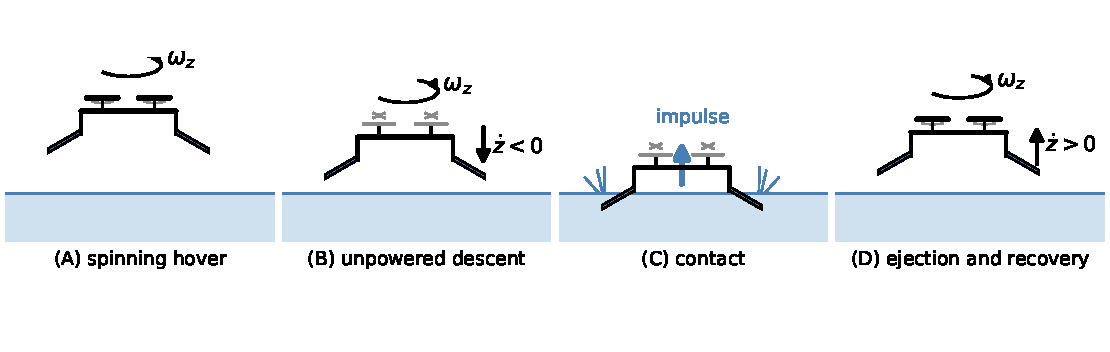
\includegraphics[width=\linewidth]{Assets/ch1fig1_hop_cycle.pdf}
    \caption{The hop cycle, in side view. \textbf{(A)} The vehicle hovers while spinning about its vertical axis at rate $\omega_z$: two rotors are mounted tangentially and drive the rotation, and two are mounted vertically and carry the lift. \textbf{(B)} The lift rotors are commanded to zero, marked by the crossed disks, and the vehicle descends unpowered; the tangential rotors keep driving the spin, so the hydrofoils reach the surface still sweeping at close to their hover speed. \textbf{(C)} The foils submerge and the water returns a large vertical impulse, braking the spin as it does so. \textbf{(D)} The vehicle leaves the surface climbing, control is restored, and the cycle repeats.}
    \label{fig:hop_cycle}
\end{figure}

\section{Related Work}
\label{sec:related_work}



\paragraph{Aquatic--aerial robots.}
Robots able to operate in both air and water have been pursued from several
directions.  One line of work develops fixed-wing vehicles that plunge into
the water and relaunch from it~\cite{siddall2014launching}, while another adapts rotorcraft to
land on, float on, or dive beneath the surface~\cite{alzubi2018loon}.  A third,
bio-inspired line mimics animals such as flying fish, diving birds, and
semi-aquatic insects that transition between swimming
and flight~\cite{zufferey2019consecutive,chen2017biologically}.

What these vehicles have in common is a difficulty of principle: the two media
make opposite demands of the same hardware.  Hydrodynamic loads at entry are
orders of magnitude larger than the aerodynamic loads the airframe is otherwise
sized for, so a structure light enough to fly must survive impacts it was not
built for.  A rotor sized to accelerate a large mass of air is badly matched to
water, which is dense enough to overload it at the same rotational speed.  And
everything that makes a vehicle amphibious, the sealing, the buoyancy, and the
structure that takes the impact, is mass the flight case carries for the whole
mission.  The usual resolution is to specialise, accepting reduced performance
in one medium or carrying a separate mechanism for the transition; in either
case water contact is treated as a destination, and the return to the air is
handled by restarting flight from rest or by a dedicated launch event.

\paragraph{Leaving the water.}
Departing the surface is the most demanding part of amphibious operation, and
the reason is a matter of scale.  The adhesive force holding a body to the
surface acts along the contact perimeter and therefore falls only linearly as
the vehicle is made smaller, while the thrust available to break it falls with
the disk area of the rotors; the ratio moves against the vehicle as it shrinks,
which is why the problem is acute at micro scale and mild at large scale.  A
departing vehicle must also accelerate the water entrained around it, adding
effective mass at precisely the moment it has none of the forward speed that
would otherwise generate lift.  It must therefore start from rest, in the worst
part of its thrust curve, against a force that does not scale in its favour.

Sustained motor power is the wrong instrument for this, and the reported
solutions all amount to releasing stored energy faster than the propulsion
system could deliver it: impulsive jumping~\cite{zufferey2019consecutive},
rapid gas generation or combustion~\cite{chen2017biologically}, or oversizing
the propulsion system so that its peak thrust suffices~\cite{alzubi2018loon}.
Each enables a transition, and each spends a large, non-recoverable share of
the energy budget doing so, which is what limits how many transitions a vehicle
can make.

\paragraph{Water-entry and skipping physics.}
The physics of objects bouncing on water has been studied independently of
robotics.  Stone-skipping and the related water-entry problem have been
analysed for both spinning and non-spinning bodies~\cite{bocquet2003physics,truscott2014water}, establishing
that a flat object striking water at a shallow angle experiences a large,
short-lived hydrodynamic reaction that can redirect it upward before it
sinks~\cite{clanet2004secrets}.

That reaction is inertial rather than buoyant.  During the contact the body
accelerates a mass of water downward and outward, and the force it feels is the
reaction to that momentum transfer; it grows with the square of the speed at
which the surface is swept and vanishes when the body is at rest.  Spin enters
this picture in two distinct ways, and the distinction matters for what
follows.  For a thrown stone, spin is stabilising: it holds the attack angle
against the torque of the impact, which would otherwise tumble the stone and
turn a skip into a splash~\cite{bocquet2003physics}.  For the vehicle described
here, spin instead supplies the sweep velocity itself, so the reaction is
available without the body having to travel horizontally across the surface at
all.  These studies characterise the conditions for a successful skip (approach
angle, speed, and spin) but consider passive, unpowered projectiles, and
neither role of spin has been examined for a controlled, self-propelled
vehicle.

\paragraph{Spinning multirotors.}
Multirotors that hover while spinning rapidly about their vertical axis have
been studied for some time, chiefly because a vehicle that gives up control of
its heading gains something in return.  Mueller and D'Andrea characterise
relaxed-hover solutions in which a multicopter sustains a constant spin rather
than holding a fixed heading, and show that abandoning yaw regulation is what
allows a quadrotor to keep flying after losing a
rotor~\cite{mueller2016relaxed}.  The SplitFlyer vehicles use the same freedom
differently, letting a quadrotor separate in flight into two bicopters, each
underactuated and able to fly only by
spinning~\cite{bai2020splitflyer,bai2022splitflyerair}.

Such vehicles are hard to control for two related reasons.  The first is that
the actuation axis rotates with the body, so a fixed differential thrust does
not produce a fixed torque in the inertial frame.  The command has to be
modulated in phase with the rotation, and any lag between measuring the yaw
angle and acting on it appears directly as an error in the direction of the
torque applied.  The second is that a body carrying large angular momentum
responds to a torque by precessing rather than by accelerating, so a torque
applied about one axis tilts the vehicle about the other, and the near-hover
intuition that roll torque produces roll no longer holds.  The standard
response is to stop describing the vehicle by its full orientation.  Yaw is
neither regulated nor of interest, only the direction of the thrust axis
matters, and that direction is a two-parameter object independent of the
instantaneous yaw angle; the gyroscopic reduced attitude dynamics written in
those two parameters are what make the problem
tractable~\cite{bai2022splitflyerair}.

In these platforms the
spin arises as a consequence of the actuator configuration: yaw torque cannot
be independently cancelled, and the vehicle settles at whatever rate balances
that residual torque.  The vehicle described here shares the fast-spin regime
and the reduced-attitude dynamics that come with it, but reaches it by different means: dedicated tangential rotors drive the rotation directly, so
the spin rate is commanded rather than inherited from the thrust balance.  This
matters because the hop depends on the tangential speed of the hydrofoils at
water contact: a spin rate that can be set is a design variable, not a
constraint to be worked around.

\paragraph{Summary.}
These bodies of work supply the individual ingredients (amphibious airframes, water-entry hydrodynamics, and control of fast-spinning multirotors) but none
combines them into a vehicle that uses spinning hydrofoils to hop repeatedly
across water, drawing the impulse that returns it to the air from the contact
itself rather than from a mechanism carried for the purpose.  That combination
is the subject of this thesis.

\section{Research Objectives}
\label{sec:research_objectives}

The goal of this thesis is to establish water-skipping as a practical mode of
locomotion for a micro aerial vehicle: to show that a small rotorcraft can
strike a water surface and be thrown back into the air by its own spinning
hydrofoils, and that it can do so repeatedly under closed-loop control.  This
goal breaks into four objectives.

\begin{enumerate}
  \item \textbf{Model the hop.}  Develop a quantitative model of the brief
    submersion phase that predicts the vertical impulse delivered to the
    vehicle as a function of the hydrofoil geometry, its attack angle, the spin
    rate at contact, and the descent velocity.  The model must be tractable
    enough to guide design decisions and to indicate which parameters dominate
    the outcome.

  \item \textbf{Design a vehicle that can survive and exploit the hop.}
    Realise an airframe that carries the hydrofoils at a useful radius, spins
    fast enough to give them the tangential speed the model requires, tolerates
    repeated water impact, and remains light enough to be ejected by the
    impulse its own foils generate.

  \item \textbf{Control a fast-spinning vehicle.}  Establish attitude and
    position control for an airframe rotating continuously about its vertical
    axis, where the spin dominates the attitude dynamics and the vehicle must
    be regulated as a rotating body rather than a heading-holding one.  The
    controller must hold station well enough to place the vehicle over a chosen
    point, execute a controlled descent onto the surface, and recover the
    vehicle after ejection.

  \item \textbf{Demonstrate the cycle experimentally.}  Show on hardware that
    the full sequence (hover, descend, contact, eject, recover) closes, and
    that the vehicle returns to controlled flight after water contact rather
    than merely surviving a single impact.
\end{enumerate}

\section{Thesis Contributions}
\label{sec:thesis_contributions}

The contributions of this thesis are as follows.

\begin{itemize}
  \item \textbf{A water-skipping locomotion mode for MAVs.}  The central
    contribution is the locomotion mode itself: a rotorcraft that hops across
    water on spinning hydrofoils, exploiting the density contrast between air
    and water so that the foils cost the vehicle little in flight yet deliver a
    large impulse during a contact lasting roughly a tenth of a second.  This treats
    water contact as a repeatable means of travel rather than as a landing, a
    dive, or a sampling stop.

  \item \textbf{A blade-element model of hydrofoil-driven ejection.}  A
    quasi-steady blade-element model of the submersion phase
    (Chapter~\ref{dynamic}) that predicts ejection velocity from foil geometry,
    attack angle, spin rate, and impact conditions, and identifies the
    parameters that govern whether a hop succeeds.

  \item \textbf{A spinning airframe with an independently commanded spin rate.}
    A vehicle design (Chapter~\ref{chapter:paperone}) in which two tangentially
    mounted rotors drive the rotation directly while two vertically mounted
    rotors provide lift and attitude authority.  Decoupling the spin from the
    lift channel turns the spin rate into a commanded design parameter, allowing
    the tangential blade speed at water contact to be set to what the hop
    requires.

  \item \textbf{Flight control at high spin rates.}  A control formulation and
    implementation (Chapter~\ref{chapter:papertwo}) that keeps the vehicle
    stable and position-controllable while spinning, together with an online
    method for separating the spin-synchronous artefact from the estimated
    attitude (Chapter~\ref{chapter:paperthree}).  In flight testing the vehicle
    remained controllable at spin rates approaching
    $10{,}000^{\circ}\,\mathrm{s^{-1}}$ without an upper limit being reached.

  \item \textbf{Experimental demonstration of repeated hops.}  Flight
    experiments (Chapter~\ref{chapter:paperthree}) demonstrating hops on a still
    water surface, including sequences in which the vehicle regains controlled
    flight after contact and returns toward its commanded height.
\end{itemize}

\section{Thesis Organization}

The remainder of this thesis is organized as follows:

\textbf{Chapter~\ref{dynamic}} develops the hydrodynamic model of the hop.  A
quasi-steady blade-element treatment of the submersion phase predicts the
forces generated by the hydrofoils as they sweep through the water, and
establishes how the resulting ejection depends on foil geometry, attack angle,
spin rate, and impact velocity.

\textbf{Chapter~\ref{chapter:paperone}} presents the design of the vehicle: the
airframe and its rotor configuration, the propulsion and power system, and the
geometry of the hydrofoils that carry out the hop.

\textbf{Chapter~\ref{chapter:papertwo}} develops the flight dynamics and
control of the spinning airframe, covering the coordinate frames and system
definition, the translational and attitude dynamics, the reduced dynamics that
apply under high yaw rate, and the controller built on them.

\textbf{Chapter~\ref{chapter:paperthree}} reports the experimental validation.
It describes the flight testing setup, an online method for separating
rotation-induced oscillations from the state estimate, and flight results for
constant-height jumping on water.

\textbf{Chapter~\ref{chapter:conclusion}} summarizes the contributions of this
thesis, discusses their implications, and outlines directions for future work.


\cleardoublepage
\chapter{Dynamic Modeling of Water-Skipping Motion}

\label{dynamic}

\section{Overview of Water-Skipping Process}

A hop is a single exchange of energy with the water surface.  The vehicle
arrives spinning and descending; it leaves spinning more slowly and rising.
Everything that makes the manoeuvre possible happens in the few tens of
milliseconds in between, and this chapter is concerned with what governs that
interval.

The mechanism rests on the vehicle's rotation.  Four hydrofoils are carried on
the airframe and turn with it, so that each sweeps a circular path at a
tangential speed $\omega r$ set by the spin rate and its radius.  That speed is
an order of magnitude larger than the vehicle's descent speed, which means the
foils meet the water almost edge-on, travelling far faster sideways than
downward.  Inclined at a fixed angle $\beta$, each foil therefore acts as a
lifting surface driven by the spin rather than by the fall.

What makes this worth doing is the density of the fluid.  The same foils sweep
through air during flight, but water is roughly three orders of magnitude
denser, so a foil that produces a negligible force in air produces a large one
the instant it is immersed.  The vehicle thus carries surfaces that cost little
in flight yet can arrest its descent on contact.

The contact itself proceeds in two competing directions.  The foils generate a
vertical force that decelerates and then reverses the vehicle, and
simultaneously a resisting torque that drains the spin which produces that
force.  A hop succeeds when the vertical impulse is large enough to return the
vehicle to the air before the spin has decayed too far to keep it controllable
once there.  The model developed in this chapter quantifies both effects: the
quasi-steady hydrodynamics of a single foil section
(Section~\ref{sec:quasi_steady}), their integration along the span
(Section~\ref{sec:blade_element}), and the coupled vertical and rotational
motion that results (Section~\ref{sec:vertical_rotational}).

\paragraph{Scope and assumptions.}
The treatment is deliberately economical.  Forces are taken as quasi-steady,
so that each instant is evaluated as if the flow were in equilibrium; the
foils are modelled as flat plates, with the separated-flow coefficients that
follow; only the submerged portion of a foil is assumed to generate force, and
the water surface is treated as flat and undisturbed, so that the wetted extent
of a foil is fixed by its geometric depth alone.  Air loads during the contact
are neglected beside the hydrodynamic ones.  These assumptions make the problem
tractable and expose the parameters that matter, at the cost of quantitative
fidelity where the free surface deforms appreciably; Chapter~\ref{chapter:paperthree}
compares the resulting predictions with flight measurements and returns to this
point.

\section{Quasi-Steady Blade-Element Model}
\label{sec:quasi_steady}

Because the density of water exceeds that of air by three orders of magnitude,
the force generated by the submerged portion of a hydrofoil dominates the
motion of the vehicle during contact, and only that force is retained here.

The foil is not a single lifting surface with one velocity.  It rotates with
the airframe, so its local speed varies along the span, and it is therefore
treated by the blade-element method: the foil is divided into elements of
radial width $dr$, each evaluated as a two-dimensional section under
quasi-steady conditions, and the element forces are integrated along the span.
The quasi-steady hydrodynamics are introduced directly at the element level
below, since that is the only level at which they are applied.

\paragraph{Element kinematics.}
Figure~\ref{fig:model_definitions}(B) shows the foil in plan view.  It occupies
an annular band of the swept disk, beginning at the root radius
$r_{\mathrm{in}}$ fixed by the motor-mount circle and extending to the tip
radius $r_{\mathrm{tip}}$; its radial span is $r_{\mathrm{tip}}-r_{\mathrm{in}}$,
and no lifting surface occupies $r<r_{\mathrm{in}}$.

An element at radius $r$ meets the water with two velocity components: a
horizontal component due to the rotation of the vehicle, and a vertical
component due to its descent.  The horizontal component is the local
tangential speed
%
\begin{equation}
    v_x(r) = \omega r ,
    \label{eq:blade_tangential_velocity}
\end{equation}
%
which varies along the span, so every quantity derived from it is a function of
$r$.  The vertical component is the descent rate $\dot{z}$, common to the whole
vehicle.  The resultant speed of the element relative to the water is therefore
%
\begin{equation}
    v(r) = \sqrt{(\omega r)^2 + \dot{z}^{\,2}} .
    \label{eq:blade_resultant_velocity}
\end{equation}
%
The angle between this resultant and the horizontal is the inflow angle
%
\begin{equation}
    \gamma(r) = \tan^{-1}\!\left(\frac{-\dot{z}}{\omega r}\right),
    \label{eq:blade_gamma}
\end{equation}
%
where $\dot{z}<0$ during the descent, so $-\dot{z}$ is the downward speed.  The
foil is mounted at a fixed inclination $\beta$ to the horizontal, so the local
angle of attack combines that inclination with the inflow direction
(Figure~\ref{fig:model_definitions}(A)):
%
\begin{equation}
    \alpha(r) = \beta + \gamma(r) .
    \label{eq:blade_alpha}
\end{equation}
%
Here $\omega$ is the angular velocity of the vehicle and $\dot{z}$ its vertical
velocity.  Since $\gamma$ depends on $r$, so does $\alpha$: the angle of attack
is largest at the root, where the tangential speed is lowest and the inflow
steepest, and approaches $\beta$ at the tip.

\paragraph{Element forces.}
Under the quasi-steady assumption each element is evaluated as if the flow
around it were in equilibrium, so the standard sectional expressions apply with
the local speed and angle of attack of \eqref{eq:blade_resultant_velocity}
and~\eqref{eq:blade_alpha}.  For a flat plate in separated flow the sectional
coefficients are
%
\begin{equation}
    C_L(\alpha) = 2 \sin{\alpha}\cos{\alpha},
    \qquad
    C_D(\alpha) = 2 \sin^2{\alpha},
    \label{eq:flat_plate_coeffs}
\end{equation}
%
which hold for a thin plate at large angle of attack, where the flow separates
at both edges and the resultant force acts normal to the
plate~\cite{bocquet2003physics,truscott2014water}.

Because the hydrofoil is a thin slanted plate, the portion submerged at penetration depth $z$ extends a length $z/\sin{\beta}$ along the chordwise (slant) direction. This wetted length grows with depth only until the plate is fully wetted, which occurs at the depth $h^{*} = c\sin{\beta}$, where $c$ is the physical chord of the foil; at greater depths the wetted length is bounded by the chord itself. The submerged chord is therefore

\begin{equation}
    c_{\mathrm{sub}} = \min\!\left(\frac{z}{\sin{\beta}},\; c\right),
    \label{eq:submerged_chord}
\end{equation}
and is the same for every blade element at a given instant. The submerged area of a blade element of radial length $dr$ is then

\begin{equation}
    dS = c_{\mathrm{sub}}\,dr .
    \label{eq:blade_area}
\end{equation}

Based on the quasi-steady assumption, the differential lift and drag generated by this blade element are

\begin{equation}
    dF_L = \frac{1}{2}\rho C_L(\alpha) v^2(r)\,c_{\mathrm{sub}}\,dr ,
    \label{eq:differential_lift}
\end{equation}

\begin{equation}
    dF_D = \frac{1}{2}\rho C_D(\alpha) v^2(r)\,c_{\mathrm{sub}}\,dr ,
    \label{eq:differential_drag}
\end{equation}
where $\rho$ is the density of water, and $C_L(\alpha)$ and $C_D(\alpha)$ are the lift and drag coefficients.

The differential vertical thrust and horizontal resistance force are obtained by decomposing the lift and drag forces:

\begin{equation}
    dT = dF_L \cos{\gamma(r)} + dF_D \sin{\gamma(r)} ,
    \label{eq:differential_thrust}
\end{equation}

\begin{equation}
    dF_R = dF_D \cos{\gamma(r)} - dF_L \sin{\gamma(r)} .
    \label{eq:differential_resistance}
\end{equation}

The horizontal resistance force produces a resisting torque about the rotational center:

\begin{equation}
    dQ = r\,dF_R
    =
    r\left(dF_D \cos{\gamma(r)} - dF_L \sin{\gamma(r)}\right).
    \label{eq:differential_torque}
\end{equation}


\section{Vertical Motion and Rotational Dynamics}
\label{sec:vertical_rotational}

The total vertical thrust and resisting torque generated by one hydrofoil are obtained by integrating the blade elements along the radial direction, over the span the foil actually occupies: from the root radius $r_{\mathrm{in}}$ to the tip radius $r_{\mathrm{tip}}$. The lower limit is consequential. Because the element force grows as $(\omega r)^2$, extending the integral inward to the axis would not add a small correction but would credit the vehicle with a stretch of foil it does not carry. The chord $c$ enters the model only as the saturation limit of the submerged chord $c_{\mathrm{sub}}$ of~\eqref{eq:submerged_chord}: in the shallow phase of the contact the wetted length is set by the penetration depth alone, while in the deeper phase it is bounded by the physical extent of the foil.

Substituting the differential lift and drag into the force decomposition, the total vertical thrust generated by one hydrofoil is

\begin{equation}
    T_{\mathrm{foil}}
    =
    \int_{r_{\mathrm{in}}}^{r_{\mathrm{tip}}}
    \frac{1}{2}\rho c_{\mathrm{sub}} v^2(r)
    \left[
    C_L(\alpha(r))\cos{\gamma(r)}
    +
    C_D(\alpha(r))\sin{\gamma(r)}
    \right] dr .
    \label{eq:total_thrust_c}
\end{equation}

Similarly, the resisting torque generated by one hydrofoil is

\begin{equation}
    Q_{\mathrm{foil}}
    =
    \int_{r_{\mathrm{in}}}^{r_{\mathrm{tip}}}
    \frac{1}{2}\rho c_{\mathrm{sub}} r v^2(r)
    \left[
    C_D(\alpha(r))\cos{\gamma(r)}
    -
    C_L(\alpha(r))\sin{\gamma(r)}
    \right] dr .
    \label{eq:total_torque_c}
\end{equation}

If the vehicle has $N$ identical hydrofoils that contact the water under the same condition, the total vertical thrust and resisting torque are approximated as

\begin{equation}
    T = N T_{\mathrm{foil}},
    \label{eq:total_vehicle_thrust}
\end{equation}

\begin{equation}
    Q = N Q_{\mathrm{foil}}.
    \label{eq:total_vehicle_torque}
\end{equation}

In practice, $N$ represents the number of effective hydrofoils in contact with the water at a given time step.

Combining the above equations, the total vertical thrust and resisting torque can be summarized as nonlinear functions of the vehicle states and hydrofoil design parameters:

\begin{align}
    T &= T\left(
        z,\dot{z},\omega,r_{\mathrm{in}},r_{\mathrm{tip}},c,\beta,N,\rho
    \right),
    \label{eq:T_function} \\[2pt]
    Q &= Q\left(
        z,\dot{z},\omega,r_{\mathrm{in}},r_{\mathrm{tip}},c,\beta,N,\rho
    \right).
    \label{eq:Q_function}
\end{align}

The vertical and rotational dynamics of the vehicle during water impact are then written as

\begin{align}
    m\ddot{z} &= \phantom{-}T\left(
        z,\dot{z},\omega,r_{\mathrm{in}},r_{\mathrm{tip}},c,\beta,N,\rho
    \right) - mg,
    \label{eq:vertical_dynamics_function} \\[2pt]
    I\dot{\omega} &= -Q\left(
        z,\dot{z},\omega,r_{\mathrm{in}},r_{\mathrm{tip}},c,\beta,N,\rho
    \right).
    \label{eq:rotational_dynamics_function}
\end{align}

In this formulation the hydrofoil geometry enters through two parameters: the root and tip radii $r_{\mathrm{in}}$ and $r_{\mathrm{tip}}$, which set the radial integration range $r_{\mathrm{in}} \le r \le r_{\mathrm{tip}}$ ($r_{\mathrm{in}}$ being fixed by the airframe and $r_{\mathrm{tip}}$ taken as the design variable), and the chord $c$, which bounds the chordwise wetting. The submerged chord $c_{\mathrm{sub}} = \min(z/\sin{\beta},\,c)$ grows with the penetration depth in the shallow phase of the contact and saturates at the physical chord once the plate is fully wetted, at depths beyond $h^{*} = c\sin{\beta}$.
\section{Simulation}
\label{sec:simulation}

The coupled vertical and rotational dynamics of~\eqref{eq:vertical_dynamics_function} and~\eqref{eq:rotational_dynamics_function} are integrated numerically through a single water contact. Starting from the instant the foils touch the surface, the state $(z,\dot{z},\omega)$ is advanced with a fixed-step semi-implicit Euler scheme until the foils leave the water, that is, until $z$ returns to the surface with an upward velocity. For a given entry condition (entry spin $\omega_0$ and downward entry velocity $\dot{z}_0$) and foil geometry (root radius $r_{\mathrm{in}}$, tip radius $r_{\mathrm{tip}}$ and inclination $\beta$), the simulation returns the two quantities that characterise the hop: the exit spin $\omega_{\mathrm{exit}}$ and the exit vertical velocity $\dot{z}_{\mathrm{exit}}$.


\paragraph{Anatomy of a hop.}
Figure~\ref{fig:hop_time_history} overlays nine simulated contacts at the as-built tip radius of $145~\mathrm{mm}$, combining three foil inclinations ($\beta = 10^\circ, 28^\circ, 45^\circ$) with three entry speeds ($\dot{z}_0 = -1, -2, -3~\mathrm{m\,s^{-1}}$), all entering at the measured spin of $\omega_0 = 8000~\mathrm{deg\,s^{-1}}$. Solid curves are the vertical velocity $\dot{z}(t)$ on the left axis, dashed curves the spin $\omega(t)$ on the right, and filled circles mark the instant the foils leave the water.

Every case in this set ejects. The descent is arrested and reversed within $3.7$--$4.9~\mathrm{ms}$, and the vehicle leaves the surface climbing at $0.8$--$2.3~\mathrm{m\,s^{-1}}$ while retaining between $79\%$ and $99\%$ of its entry spin. The ordering is systematic: within each group of three, a faster entry produces a larger hop, and across the groups a steeper foil produces a longer contact and a heavier spin loss. The shallow $\beta = 10^\circ$ contacts give up almost no spin at all, while the steep $\beta = 45^\circ$ contact at the fastest entry surrenders a fifth of it.

Two features of the traces carry the physics. First, the reversal is not symmetric: each velocity curve turns sharply upward and then flattens as it approaches the surface, because the spin that generates the lift is itself being consumed. Second, the spin curves fall monotonically and never recover during the contact; whatever is spent is spent for good, and must be restored by the rotors during the flight that follows. The water contact is therefore not a conservative bounce. Its role is to \emph{reverse the vertical velocity and return the vehicle to the air with enough spin left to be controllable}, and the balance between those two demands is what the design study below quantifies.

\begin{figure}[t]
    \centering
    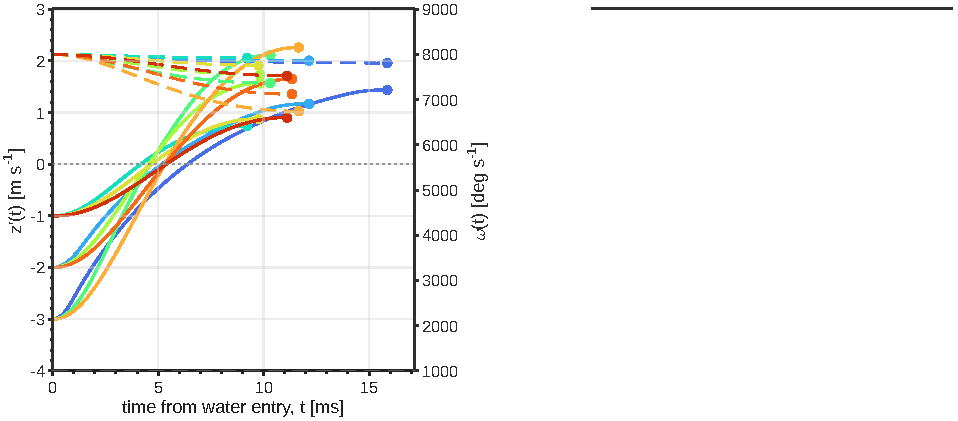
\includegraphics[width=\linewidth]{Assets/ch2fig1_hop_trajectories.pdf}
    \caption{Simulated time histories of nine water contacts at the as-built tip radius $r_{\mathrm{tip}} = 145~\mathrm{mm}$ and root radius $r_{\mathrm{in}} = 75~\mathrm{mm}$, combining three inclinations ($\beta = 10^\circ, 28^\circ, 45^\circ$) with three entry speeds ($\dot{z}_0 = -1, -2, -3~\mathrm{m\,s^{-1}}$), all entering at $\omega_0 = 8000~\mathrm{deg\,s^{-1}}$. Solid curves: vertical velocity $\dot{z}$ (left axis). Dashed curves: spin $\omega$ (right axis). Filled circles mark water exit. All nine contacts eject; steeper inclination and faster entry both lengthen the contact and increase the spin surrendered to the water.}
    \label{fig:hop_time_history}
\end{figure}

\paragraph{Design space and the hop--spin trade-off.}
Evaluating the model across the space spanned by the inclination $\beta$, the tip radius $r_{\mathrm{tip}}$, and the entry velocity $\dot{z}_0$ shows how the two hop metrics respond to the design. Figure~\ref{fig:design_space_maps} plots every simulated design as a point in this space, coloured by the exit vertical velocity $\dot{z}_{\mathrm{exit}}$ (left, the hop) and by the exit spin $\omega_{\mathrm{exit}}$ (right, the spin retained for the flight that follows). Across the space the hop ranges from $0.36$ to $3.17~\mathrm{m\,s^{-1}}$ and the retained spin from $4159$ to $7980~\mathrm{deg\,s^{-1}}$, between $52\%$ and essentially all of the entry spin.

The two panels are organised by different variables, and the contrast is the substance of the figure. The hop follows the entry velocity above all: the left panel is layered almost entirely along the $\dot{z}_0$ axis, and holding the geometry fixed while varying the entry speed alone moves $\dot{z}_{\mathrm{exit}}$ by $85\%$ of its range. The inclination $\beta$ is the second lever, worth a further $37\%$; a steeper foil presents more of its area to the flow and turns more of the sweep into vertical impulse. The tip radius is nearly inert by comparison, changing the hop by only about $4\%$ across a two-fold change in radius, because at the sweep speeds considered here the foils already generate far more force than is needed to reverse the descent, and the contact ends before the extra radius can express itself.

The retained spin behaves in the opposite sense. It is largest, close to the full entry value, where the foils do least work: shallow inclination and gentle entry. It falls steadily as either the inclination steepens or the entry speed rises, reaching $52\%$ at the most heavily loaded corner of the space. The two objectives therefore oppose one another: within this model the largest hop, $3.17~\mathrm{m\,s^{-1}}$, occurs at $\beta = 42^{\circ}$ and the fastest entry considered, and costs a quarter of the spin, while the design that retains all of its spin delivers a hop of only $0.36~\mathrm{m\,s^{-1}}$.

This is the compromise that sizes the vehicle: take as much hop as can be had while leaving enough spin for the vehicle to remain controllable on exit. It also indicates where design effort is repaid. The inclination and the conditions of entry govern the outcome, whereas the radial extent of the foil, once large enough, does not, so the foil may be sized by structural and packaging considerations without penalising the hop. The geometry selected on this basis is described in Chapter~\ref{chapter:paperone}.

\begin{figure}[t]
    \centering
    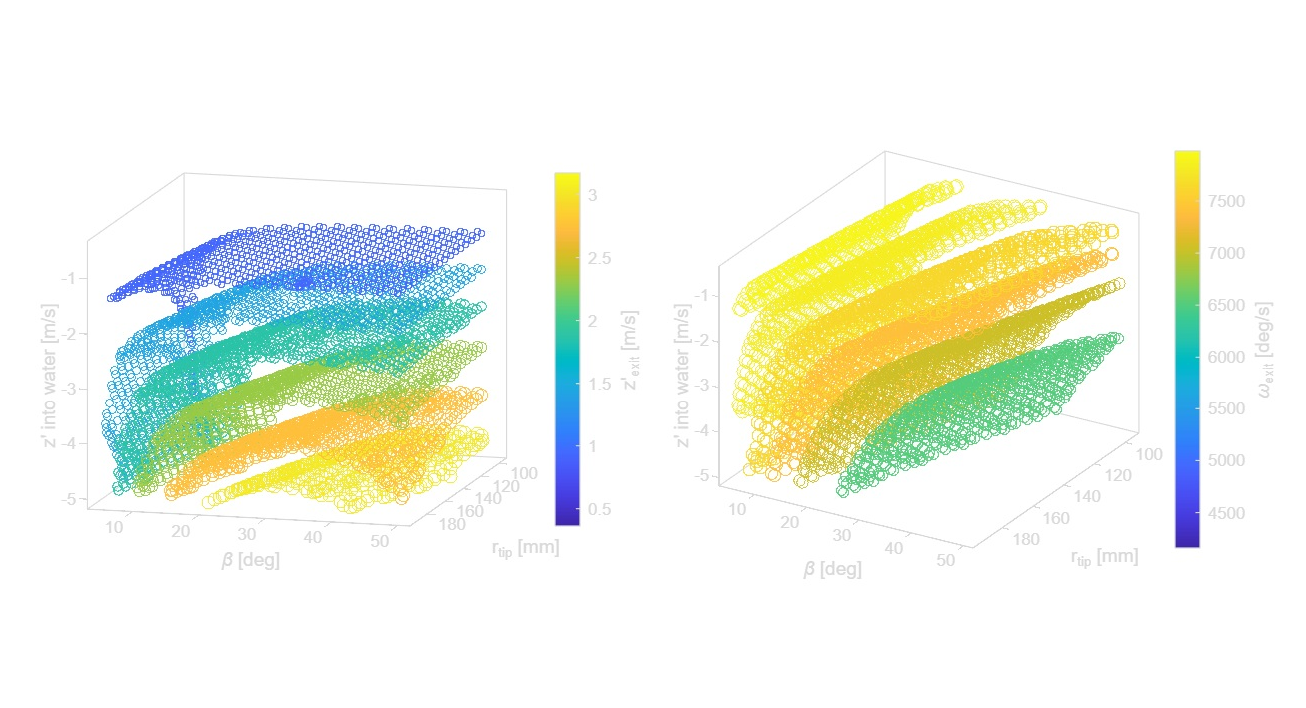
\includegraphics[width=\linewidth]{Assets/ch2fig2_design_space.pdf}
    \caption{Hop performance over the design space $(\beta,\ r_{\mathrm{tip}},\ \dot{z}_0)$, evaluated at the as-built root radius $r_{\mathrm{in}} = 75~\mathrm{mm}$ and entry spin $\omega_0 = 8000~\mathrm{deg\,s^{-1}}$. Each point lies on an iso-value surface of the response, coloured by the exit vertical velocity $\dot{z}_{\mathrm{exit}}$ (left, the hop) and by the exit spin $\omega_{\mathrm{exit}}$ (right, the retained spin). The two responses are organised by different variables: the hop is layered along the entry velocity and, secondarily, the inclination, while the retained spin falls wherever the foils are most heavily loaded. Both are nearly independent of the tip radius over the range shown.}
    \label{fig:design_space_maps}
\end{figure}

\cleardoublepage
\chapter{Design of the Water-Skipping MAV}
\label{chapter:paperone}

\section{Design Requirements}
\label{sec:design_requirements}

The vehicle must satisfy two coupled sets of requirements: it must generate
enough lift to hover as a quadrotor, and its spinning hydrofoils must produce
sufficient hydrodynamic impulse during a brief water-surface contact to eject
it back into the air.

\paragraph{Flight requirements.}
The complete vehicle, including motion-capture markers and assembly
adhesive, has an all-up mass of $m = 90\;\mathrm{g}$.  Yaw torque is
generated by two mechanisms acting in the same rotational sense.  Two of
the four rotors are mounted horizontally, tangential to the frame, and are
driven at a fixed thrust setpoint that is set independently of the
vertical-lift channel; this direct tangential thrust is the dominant
driving torque.  The remaining two rotors are mounted vertically and
provide lift and attitude authority; because all four rotors turn in the
same physical direction, their reaction torque adds to, rather than
cancels, the tangential drive torque, contributing a secondary,
thrust-coupled term (Section~\ref{sec:mech_design}).  Because the dominant
tangential term is commanded independently of the lift channel, the
resulting spin rate is a tunable operating parameter rather than a fixed
consequence of the vehicle's thrust or airframe drag.  The attitude
controller runs at a loop rate of
$100\;\mathrm{Hz}$; a na\"ive requirement of several control updates per
revolution would place a ceiling near $\omega_z^* < 20\pi\;\mathrm{rad\,s^{-1}}$
($\approx 3600^{\circ}\,\mathrm{s^{-1}}$), but flight testing has reached
spin rates approaching $10{,}000^{\circ}\,\mathrm{s^{-1}}$ without
encountering a controllability limit.  This indicates that closed-loop
latency across the estimation, control, and actuation pipeline, not the raw number of control updates per revolution, is the more relevant constraint
on controllability at high spin rate; this relationship was not
systematically characterised in the present work and is identified as a
direction for future study (Chapter~\ref{chapter:conclusion}).  The four
rotors are driven from a $4\mathrm{S}$ high-voltage lithium polymer battery
(Coddar CD4S35090HV; \SI{15.2}{V} nominal, \SI{350}{mAh}, \SI{5.32}{Wh}, 90C
continuous discharge), supplying four Sparis \mbox{1204} motors rated at
$4{,}500\;\mathrm{KV}$.

\paragraph{Water-skipping requirements.}
For a successful hop the hydrofoils must, during the brief submersion phase,
generate a net vertical impulse large enough to reverse the vehicle's downward
velocity and return it to free flight.  Blade-element simulation of the
submersion dynamics (described in Chapter~\ref{dynamic}) shows that
both the hydrofoil inclination angle $\beta$ and the spin rate $\omega_z$
at water contact are primary drivers of the ejection velocity; the design
therefore cannot be finalised independently of the flight dynamics.

\section{Overall Mechanical Design}
\label{sec:mech_design}

% =====================================================================
% FIGURE SLOT 3.1 -- ANNOTATED VEHICLE PHOTOGRAPH  [you supply]
% Source: test results raw material/videos/photos/DSC00963.JPG (3/4 view)
% Annotate: the two tangential rotors, the two lift rotors, one hydrofoil
% leg, the Bolt board, the battery, and a mocap marker.
% To fill: delete the \fbox{...} block and uncomment the \includegraphics.
% =====================================================================
\begin{figure}[t]
    \centering
    % TODO(annotate): add callouts -- tangential rotors, lift rotors, one
    % hydrofoil leg, Bolt board, battery, mocap marker.
    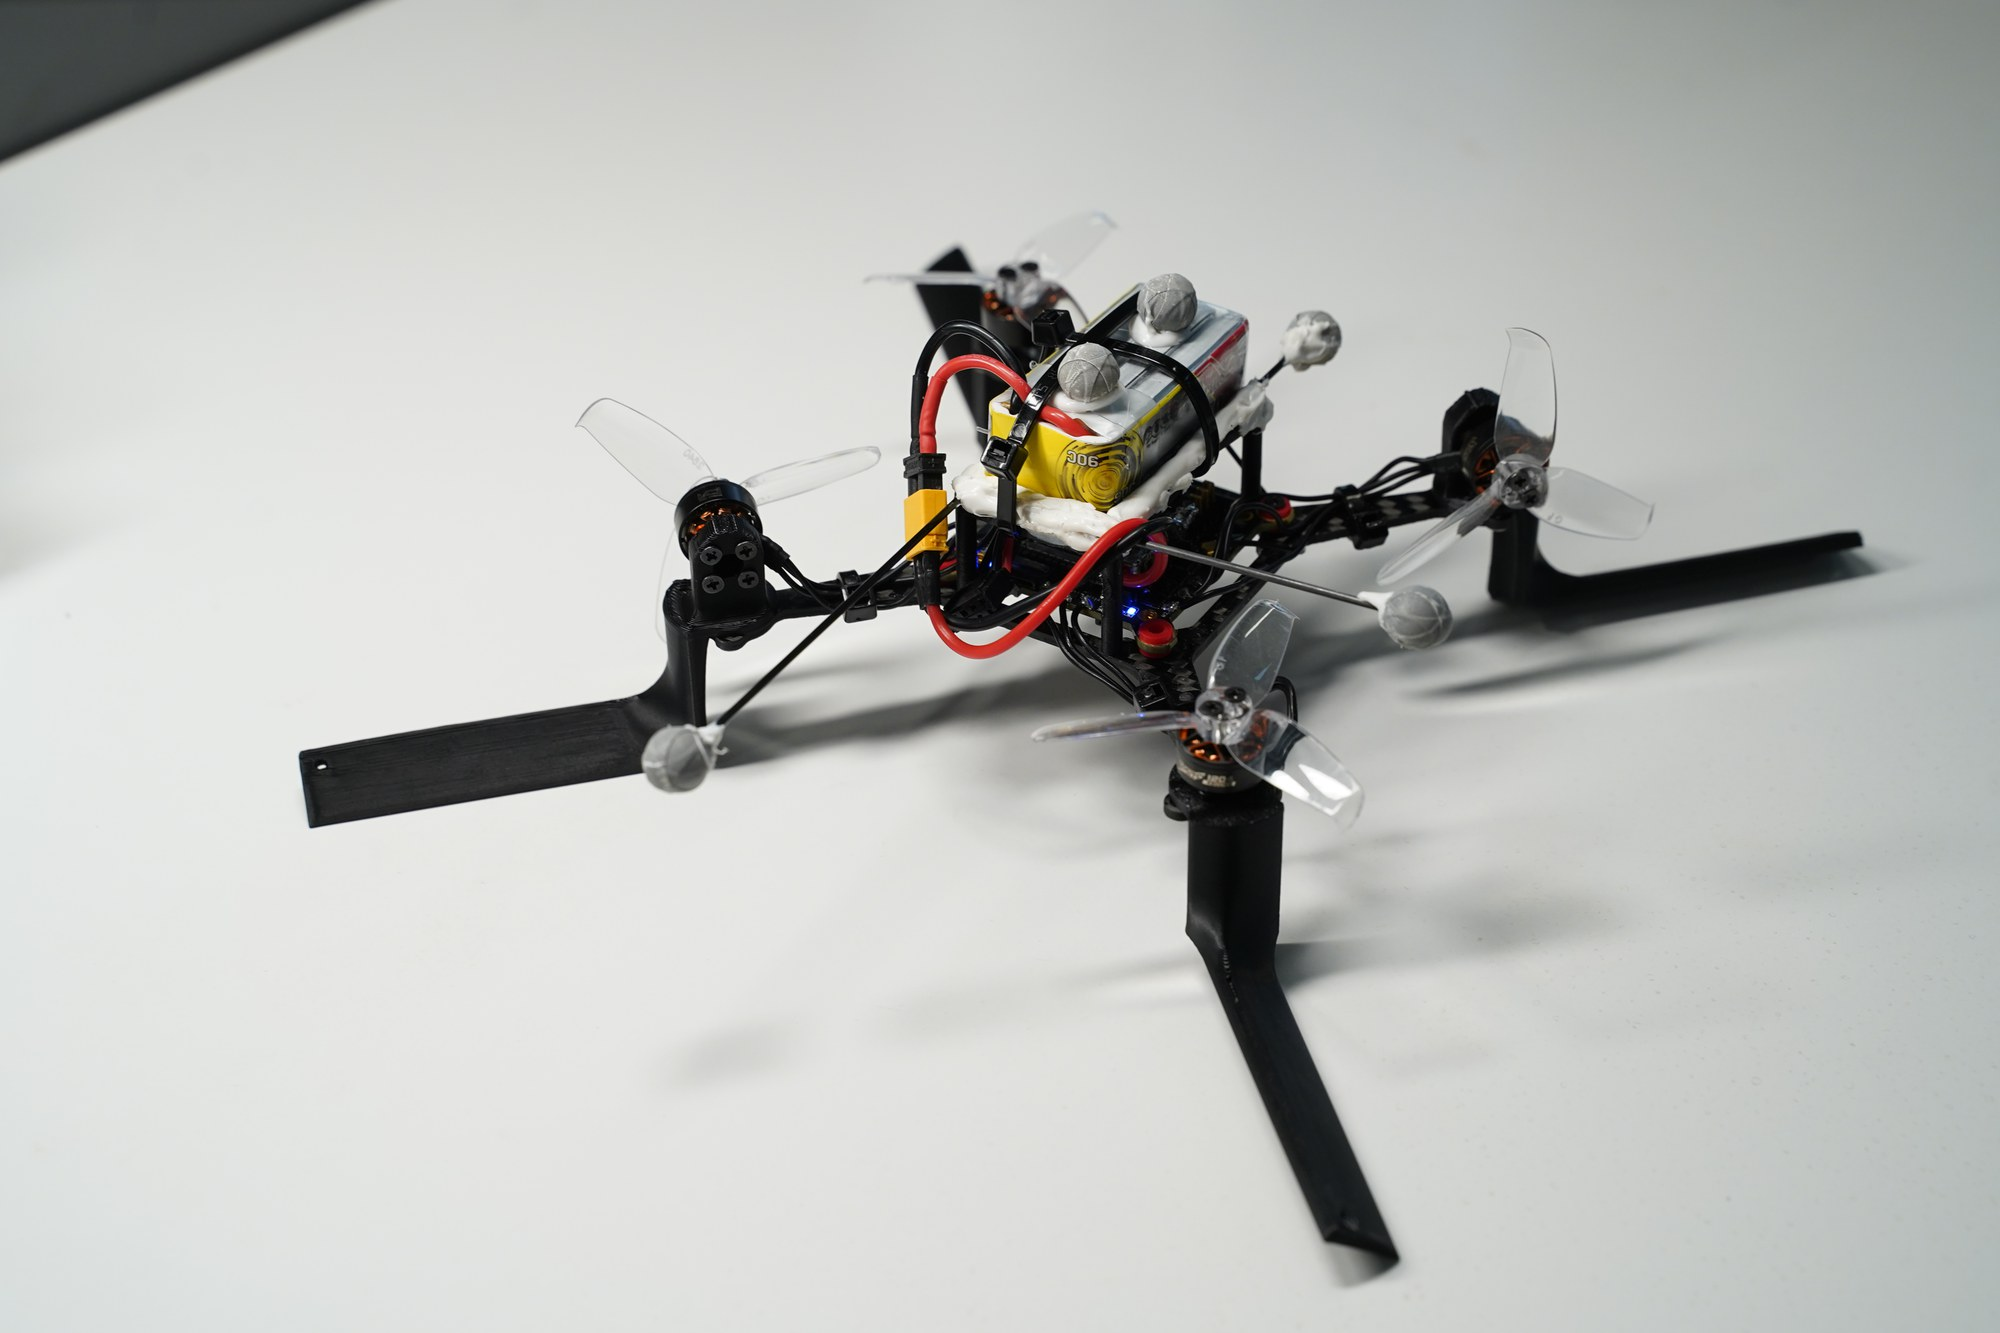
\includegraphics[width=0.85\linewidth]{Assets/ch3fig1_vehicle.jpg}
    \caption{The as-built water-skipping MAV.  Two rotors are mounted
    vertically and provide lift and attitude authority; two are mounted
    horizontally, tangential to the frame, and drive the rotation.  Each of
    the four motor mounts carries a moulded leg that drops below the airframe
    and turns outward into a hydrofoil.}
    \label{fig:vehicle_photo}
\end{figure}

\paragraph{Frame and propulsion.}
The frame carries a core of diameter $150\;\mathrm{mm}$, i.e.\ a radius of
$75\;\mathrm{mm}$ from the vehicle centre to the point where each hydrofoil
assembly begins.  Four Sparis \mbox{1204} motors, rated at
$4{,}500\;\mathrm{KV}$, are installed at this radius: two are mounted
vertically and provide lift and attitude authority, and two are mounted
horizontally, tangential to the frame, and provide yaw-drive thrust only
(Section~\ref{sec:design_requirements}).  Each motor drives a Flash
\mbox{2540-3} three-blade propeller (clear polycarbonate, T-mount).% TODO:
confirm exact azimuthal placement of the vertical vs.\ horizontal motors
for the as-built frame.

\paragraph{Electronics.}
The flight controller is a Crazyflie Bolt board, which integrates a
six-axis IMU, a radio transceiver, and motor drivers on a single compact
module.  Power is supplied by a $4\mathrm{S}$ high-voltage lithium polymer
battery (Coddar CD4S35090HV; \SI{15.2}{V} nominal, \SI{350}{mAh},
\SI{5.32}{Wh}, 90C continuous discharge).  The complete vehicle, including
motion-capture markers and assembly adhesive, has an all-up mass of
$m = 90\;\mathrm{g}$.

\paragraph{Hydrofoil mounting.}
At each of the four motor mounts, a single moulded leg drops vertically from
the frame and then kinks outward into the hydrofoil itself, so that each
hydrofoil is an integral extension of its leg rather than a separate attached part, an arrangement resembling a mosquito's legs resting on a
water surface.  The horizontal, outward-kinked span of each hydrofoil
begins at the $75\;\mathrm{mm}$ motor-mount radius and extends a further
$70\;\mathrm{mm}$, so the hydrofoil tip reaches a radius $r_f = 75 + 70 =
145\;\mathrm{mm}$ from the vehicle centre, giving an overall vehicle
diameter of $290\;\mathrm{mm}$ tip-to-tip.  The four-leg assembly rotates
with the vehicle at yaw rate $\omega_z$, as described in
Section~\ref{sec:attitude_dynamics}.

% =====================================================================
% FIGURE SLOT 3.2 -- GEOMETRY DIAGRAM  [you supply, vector/CAD]
% Two views. TOP: the 75 mm motor-mount radius, the 70 mm foil span, the
% 145 mm tip radius and the 290 mm overall diameter, with the four legs and
% the vertical/tangential rotor positions marked.
% SIDE: the leg dropping from the mount and kinking outward, showing the
% 30 deg foil inclination and the drop below the airframe.
% Base layer available: videos/photos/DSC00970.JPG (top-down, unobstructed).
% =====================================================================
\begin{figure}[t]
    \centering
    % TODO(annotate): overlay dimensions on this top-down photo -- 75 mm
    % mount radius, 70 mm foil span, 145 mm tip radius, 290 mm overall.
    % A side view still needs to be drawn and added as panel (B).
    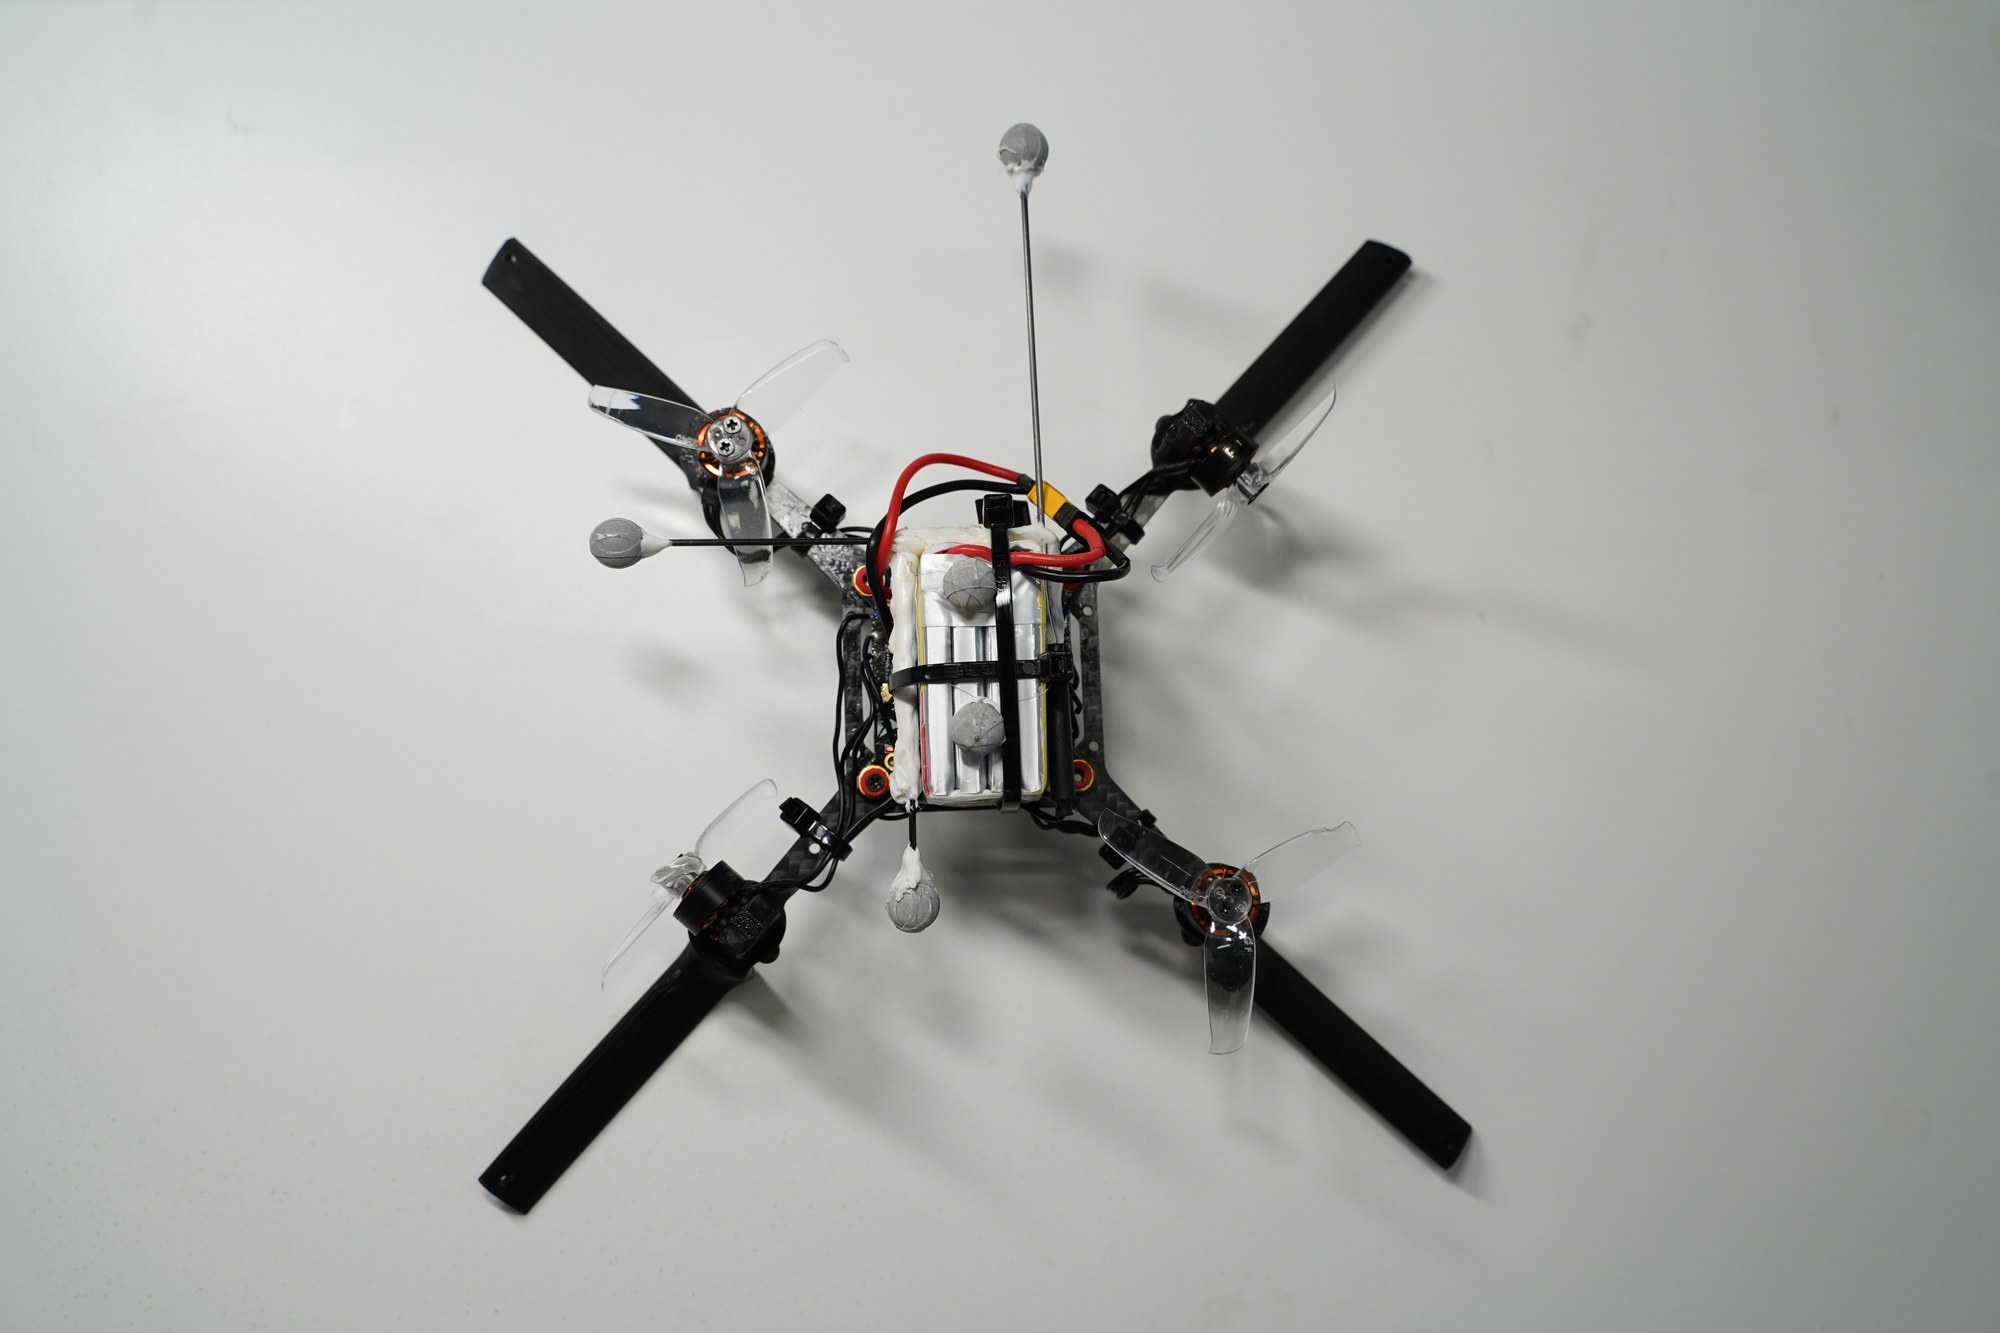
\includegraphics[width=0.85\linewidth]{Assets/ch3fig2_geometry.jpg}
    \caption{Vehicle geometry.  \textbf{(A)} Top view, showing the
    $75\;\mathrm{mm}$ motor-mount radius at which each hydrofoil begins, the
    $70\;\mathrm{mm}$ foil span, and the resulting $145\;\mathrm{mm}$ tip
    radius, giving $290\;\mathrm{mm}$ overall.  \textbf{(B)} Side view,
    showing a leg dropping from its motor mount and turning outward into the
    hydrofoil, inclined at $\beta = 30^{\circ}$ to the horizontal.}
    \label{fig:vehicle_geometry}
\end{figure}

\section{Hydrofoil Geometry}
\label{sec:foil_design}

\paragraph{Hydrofoil profile and planform.}
Each hydrofoil is a thin flat plate of thickness $3\;\mathrm{mm}$, chosen for
simplicity of fabrication and because the flat-plate hydrodynamic model
(lift coefficient $C_L = 2\sin\alpha\cos\alpha$, drag coefficient $C_D =
2\sin^2\alpha$) provides a closed-form basis for the blade-element
simulation of Chapter~\ref{dynamic}.  The foil has its own radial
length $L_f = 70\;\mathrm{mm}$, mounted with its root at the
$75\;\mathrm{mm}$ frame radius and its tip reaching $r_f = 145\;\mathrm{mm}$
from the vehicle centre (Section~\ref{sec:mech_design}), and is parametrised
by its chord $c_f$ (the dimension tangential to the sweep direction).  The
fabricated hydrofoil has chord $c_f = 15\;\mathrm{mm}$, giving a rectangular
planform area $S_f = c_f\, L_f = 1{,}050\;\mathrm{mm}^2$.

\paragraph{Attack angle.}
The hydrofoil is mounted at a fixed attack angle $\beta$ relative to the
horizontal plane, with its angled face oriented to strike the water surface
directly.  Candidate values $\beta \in \{5^{\circ}, 10^{\circ}, 15^{\circ},
20^{\circ}, 25^{\circ}, 30^{\circ}\}$ were evaluated in the blade-element
simulation of Chapter~\ref{dynamic} against predicted ejection
velocity and hop height, but only $\beta = 30^{\circ}$ was fabricated and
flight-tested; the fabricated hydrofoil is fixed at $\beta = 30^{\circ}$
with no active or passive attack-angle mechanism.  Experimental validation
of the remaining simulated angles is left to future work
(Chapter~\ref{chapter:conclusion}).

% =====================================================================
% FIGURE SLOT 3.3 -- HYDROFOIL CLOSE-UP  [you supply]
% A single leg/foil filling the frame, ideally against a plain background
% with a scale reference. Should make the 15 mm chord, the 3 mm thickness
% and the 30 deg inclination readable, and show that the leg and foil are
% one moulded part rather than an assembly.
% =====================================================================
\begin{figure}[t]
    \centering
    %\includegraphics[width=0.7\linewidth]{Assets/ch3fig3_hydrofoil.jpg}
    \fbox{\begin{minipage}[c][40mm][c]{0.7\linewidth}\centering\itshape
        Figure pending: hydrofoil close-up
    \end{minipage}}
    \caption{A single hydrofoil.  The leg and the foil are one moulded part:
    the leg drops vertically from the motor mount and turns outward into a
    flat plate of $15\;\mathrm{mm}$ chord and $3\;\mathrm{mm}$ thickness, held
    at $30^{\circ}$ to the horizontal.}
    \label{fig:hydrofoil_closeup}
\end{figure}

\section{Structural Analysis of the Hydrofoils}
\label{sec:foil_fea}

\todobox{structural analysis, or cut this section}{%
This section is a stub. Either carry out the finite-element work outlined
below, or delete the section: an empty heading is worse than no heading. For
a conference submission the argument does not depend on it, and the foils
survived every flight reported in Chapter~\ref{chapter:paperthree}, which is
itself the relevant evidence. Recommend cutting unless the analysis is
already in hand.}

% TODO: ANSYS FEA of the candidate hydrofoil geometries.
% Loads: peak water-impact distributed pressure extracted from the
%   blade-element model (Chapter~\ref{dynamic}); root clamped at mount.
% Static structural: max von Mises vs yield (safety factor); tip deflection
%   as fraction of chord (justifies the rigid-foil assumption in the BEM model).
% Modal: first natural frequencies vs spin/impact excitation.
% Geometry + material sweep -> stiffness/strength/mass trade table feeding
%   the foil-set selection in Section~\ref{sec:foil_design}.

\cleardoublepage
\chapter{Flight Dynamics and Control}
\label{chapter:papertwo}

\section{Coordinate Frames and System Definition}
\label{sec:coord_frames}

This chapter presents the flight dynamics and control framework for the
vehicle.  Its defining feature is that the airframe \emph{rotates continuously
about its vertical axis} while flying.  Two of the four rotors are mounted
horizontally, tangential to the frame, and drive this rotation directly at a
commanded thrust setpoint; the other two are mounted vertically and provide
lift and attitude authority.  All four turn in the same physical direction, so
the reaction torque of the lift rotors adds to the tangential drive rather than
cancelling it.  The vehicle therefore sustains a large, persistent yaw rate by
design---and, because the tangential rotors are commanded independently of the
lift channel, at a rate that is set rather than inherited from the thrust
balance.  This sustained rotation is what shapes the dynamics and motivates the
gyroscopic analysis that follows.

\paragraph{Inertial and body frames.}
The right-handed inertial frame $(\hat{x}^w, \hat{y}^w, \hat{z}^w)$ is
fixed to the ground with $\hat{z}^w$ pointing vertically upward.  The
position of the vehicle's centre of mass (COM) in this frame is
$\boldsymbol{p} = [x,\,y,\,z]^{\top}$.  The right-handed body frame
$(\hat{x}^b, \hat{y}^b, \hat{z}^b)$ is rigidly attached to the vehicle with
its origin at the COM; the $\hat{z}^b$ axis is aligned with the common
thrust axis of the four propellers.  The rotation matrix
$\boldsymbol{R}\in SO(3)$ maps body-frame vectors to the inertial frame,
so the world-frame direction of the thrust axis is $\boldsymbol{R}\hat{e}_3$,
where $\hat{e}_3 = [0,0,1]^{\top}$.  The body angular velocity expressed in
the body frame is $\boldsymbol{\omega} = [\omega_x, \omega_y, \omega_z]^{\top}$.
The yaw angle $\psi$ is defined as the rotation of $\hat{x}^b$ about
$\hat{z}^w$ relative to $\hat{x}^w$.

\paragraph{Non-revolving frame.}
Because the vehicle spins at high yaw rate, a non-revolving intermediate
frame $(\hat{x}^m, \hat{y}^m, \hat{z}^b)$ is introduced to describe the
attitude of the spinning disk independently of the instantaneous yaw
angle~\cite{bai2022splitflyerair}.  Under the small-inclination assumption
$|\alpha_x|, |\alpha_y| \ll 1$, the reduced attitude state
$\boldsymbol{\eta} = [\alpha_x, \alpha_y]^{\top}$ parametrises the deviation
of $\hat{z}^b$ from vertical, and the non-revolving axes are approximated as
\begin{equation}
    \hat{x}^m \approx [1,\;0,\;{-\alpha_y}]^{\top},
    \qquad
    \hat{y}^m \approx [0,\;1,\;\alpha_x]^{\top}.
    \label{eq:nm_frame}
\end{equation}
The pair $(\hat{x}^m, \hat{y}^m)$ spans the horizontal plane for any yaw
angle $\psi$; this frame is the natural setting for the gyroscopic reduced
attitude dynamics derived in Section~\ref{sec:reduced_dynamics}.

\paragraph{Rotor geometry and roles.}
The four rotors sit at equal arm length $l$ from the COM, at the body-frame
positions
\begin{equation}
    \boldsymbol{l}_1 = -\boldsymbol{l}_3
        = \frac{l}{\sqrt{2}}\!\left(\hat{x}^b + \hat{y}^b\right),
    \qquad
    \boldsymbol{l}_2 = -\boldsymbol{l}_4
        = \frac{l}{\sqrt{2}}\!\left(\hat{x}^b - \hat{y}^b\right),
    \label{eq:prop_locs}
\end{equation}
but they serve two distinct functions.  Rotors $1$ and $3$ are mounted with
their axes along $+\hat{z}^b$ and produce the \emph{lift thrusts}
$f_{1,p}, f_{3,p} \geq 0$ that support the vehicle and, through their
difference, tilt it.  Rotors $2$ and $4$ are mounted with their axes in the
body horizontal plane, oriented tangentially, and produce thrusts
$f_{2,p}, f_{4,p} \geq 0$ that act at moment arm $l$ about $\hat{z}^b$ and so
contribute only yaw torque.

The yaw torque therefore has two contributions in the same sense.  The
tangential rotors supply
\begin{equation}
    \tau_{z,\mathrm{tan}} = l\,(f_{2,p} + f_{4,p}),
    \label{eq:yaw_tangential}
\end{equation}
while each lift rotor contributes its aerodynamic reaction torque
$c\,f_{i,p}$ about $\hat{z}^b$, where $c > 0$ is the thrust-to-drag ratio
common to rotors sharing a spin direction.  Since the lift rotors turn in the
same direction as the tangential pair, these reaction torques add:
\begin{equation}
    \tau_z = \underbrace{l\,(f_{2,p} + f_{4,p})}_{\text{commanded}}
             + \underbrace{c\,(f_{1,p} + f_{3,p})}_{\text{reaction}}.
    \label{eq:yaw_torque}
\end{equation}
The first term dominates and is commanded directly: the tangential thrusts are
held at a fixed setpoint independent of the lift channel, so the spin rate is
selected rather than inherited.  The second term is a residual that varies
with the lift demand.  Because both terms drive the vehicle the same way, no
cancellation is available and no yaw equilibrium need be sought---the vehicle
spins because it is driven to, and $\omega_z$ is treated throughout this
chapter as a known, approximately constant operating parameter, measured in
flight and set by the choice of tangential thrust.

The total lift acting along $\hat{z}^b$ is carried by the vertical pair alone,
\begin{equation}
    F = f_{1,p} + f_{3,p},
    \label{eq:total_thrust_def}
\end{equation}
since the tangential rotors produce no component along the thrust axis.

\paragraph{Inertia and drag.}
By design, mass is distributed symmetrically about the $\hat{z}^b$ axis so
that the moments of inertia about roll and pitch are approximately equal,
$I_x \approx I_y \equiv I_d$.  The full inertia tensor is therefore
\begin{equation}
    \boldsymbol{I} = \mathrm{diag}(I_d,\;I_d,\;I_z),
    \label{eq:inertia}
\end{equation}
which is the axisymmetric condition required to treat the vehicle as a
gyroscope in Section~\ref{sec:reduced_dynamics}.  Rotor-induced drag is
characterised by the coefficient matrix
$\boldsymbol{B} = \mathrm{diag}(B_h, B_h, B_v)$, and aerodynamic body
damping by $\boldsymbol{D} = \mathrm{diag}(D_h, D_h, D_v)$, where subscripts
$h$ and $v$ denote horizontal and vertical components
respectively~\cite{bai2022splitflyerair}.  The vehicle mass is $m = 90\;\mathrm{g}$;
remaining hardware parameters are specified in Chapter~\ref{chapter:paperone}.

\paragraph{Propeller aerodynamic model.}
Each propeller $i$ spins about its own thrust axis at blade speed $\Omega_i$,
which is distinct from and substantially larger than the vehicle yaw rate
$\omega_z$.  The propulsive thrust follows the standard aerodynamic model
\begin{equation}
    f_{i,p} = k_f\,\Omega_i^2,
    \label{eq:thrust_model}
\end{equation}
where $k_f > 0$ is a propeller constant.  The hydrofoils are treated as
aerodynamically inert in air: they are thin flat plates carried at a fixed
inclination for water entry, not lifting surfaces, and the forces they generate
while sweeping through air are negligible beside the propeller thrust.  Their
aerodynamic role is confined to the brief submersion phase, where the working
fluid is water and the resulting forces are three orders of magnitude larger
(Chapter~\ref{dynamic}).

\section{Translational Dynamics}
\label{sec:translational_dynamics}

Treating the vehicle as a rigid body of mass $m$, Newton's second law gives
\begin{equation}
    m\ddot{\boldsymbol{p}} = \boldsymbol{R}\sum_{i=1}^{4}\boldsymbol{f}_i
        - mg\hat{e}_3,
    \label{eq:trans_eom}
\end{equation}
where the total force from propeller $i$ is
\begin{equation}
    \boldsymbol{f}_i = \hat{e}_3 f_{i,p} + \boldsymbol{f}_{i,d}.
    \label{eq:prop_force}
\end{equation}
The propulsive thrust $f_{i,p}$ is directed along the body $\hat{z}^b$ axis.
The rotor-induced drag $\boldsymbol{f}_{i,d}$, modelled as a linear function
of the air velocity at the propeller disk~\cite{bai2022splitflyerair}, is
\begin{equation}
    \boldsymbol{f}_{i,d} = -\boldsymbol{B}
        \!\left(\boldsymbol{R}^{-1}\dot{\boldsymbol{p}}
        + \boldsymbol{\omega}\times\boldsymbol{l}_i\right),
    \label{eq:rotor_drag}
\end{equation}
where the first term accounts for the translational velocity of the vehicle
and the second for the velocity of the propeller hub due to body rotation.

\paragraph{Cancellation of rotation-induced drag.}
The symmetry of the X-configuration---$\boldsymbol{l}_1 + \boldsymbol{l}_2
+ \boldsymbol{l}_3 + \boldsymbol{l}_4 = \mathbf{0}$, which follows
immediately from~\eqref{eq:prop_locs}---ensures that the rotation-induced
drag terms cancel when summed:
\begin{equation}
    \sum_{i=1}^{4}\left(\boldsymbol{\omega}\times\boldsymbol{l}_i\right)
        = \boldsymbol{\omega}\times\sum_{i=1}^{4}\boldsymbol{l}_i
        = \mathbf{0}.
    \label{eq:drag_cancel}
\end{equation}
This cancellation holds regardless of propeller spin direction and therefore
applies equally to our vehicle.  Substituting into~\eqref{eq:trans_eom}:
\begin{equation}
    m\ddot{\boldsymbol{p}}
        = \boldsymbol{R}\hat{e}_3 F
          - 4\boldsymbol{R}\boldsymbol{B}\boldsymbol{R}^{-1}\dot{\boldsymbol{p}}
          - mg\hat{e}_3.
    \label{eq:trans_full}
\end{equation}
The second term is a translational damping force present in all multirotor
vehicles.  For non-aggressive near-hover flight it is small relative to
gravity and is neglected in what follows~\cite{bai2022splitflyerair}, yielding
\begin{equation}
    m\ddot{\boldsymbol{p}} \approx \boldsymbol{R}\hat{e}_3 F - mg\hat{e}_3.
    \label{eq:trans_hover}
\end{equation}

\paragraph{Near-hover linearisation.}
For small inclinations $|\alpha_x|,|\alpha_y|\ll 1$, the body $\hat{z}^b$
axis expressed in the inertial frame is approximately
\begin{equation}
    \boldsymbol{R}\hat{e}_3 \approx
        \begin{bmatrix} J\boldsymbol{\eta} \\ 1 \end{bmatrix},
    \qquad
    J = \begin{bmatrix} 0 & 1 \\ -1 & 0 \end{bmatrix},
    \label{eq:zb_approx}
\end{equation}
where $J$ is the $-90^{\circ}$ rotation matrix in the horizontal plane.
Splitting~\eqref{eq:trans_hover} into horizontal and vertical components
and using the hover thrust condition $F\approx mg$ for the horizontal term
gives
\begin{align}
    m\ddot{\boldsymbol{p}}_2 &= mg\,J\boldsymbol{\eta},
    \label{eq:horiz_dyn}\\
    m\ddot{z} &= F - mg,
    \label{eq:vert_dyn}
\end{align}
where $\boldsymbol{p}_2 = [x,\,y]^{\top}$ is the horizontal position.
Equation~\eqref{eq:horiz_dyn} shows that horizontal acceleration is driven
solely by the vehicle tilt $\boldsymbol{\eta}$, and forms the basis of the
position controller in Section~\ref{sec:controller}.

\section{Attitude Dynamics}
\label{sec:attitude_dynamics}

The rotational motion is governed by Euler's equations in the body frame.
The angular momentum equation is
\begin{equation}
    \boldsymbol{I}\dot{\boldsymbol{\omega}}
        + \boldsymbol{\omega}\times\boldsymbol{I}\boldsymbol{\omega}
        = \sum_{i=1}^{4}\boldsymbol{\tau}_i
          + \boldsymbol{\tau}_s,
    \label{eq:euler}
\end{equation}
where $\boldsymbol{\tau}_i$ is the net torque produced by propeller $i$
at the centre of mass, and $\boldsymbol{\tau}_s = -\boldsymbol{D}\boldsymbol{\omega}$
is the aerodynamic body damping.

\paragraph{Propeller torques.}
The total torque from propeller $i$ decomposes into a thrust-induced
component and a drag-induced component:
\begin{equation}
    \boldsymbol{\tau}_i = \boldsymbol{\tau}_{i,p} + \boldsymbol{\tau}_{i,d}.
    \label{eq:prop_torque_decomp}
\end{equation}
For the two lift rotors ($i \in \{1,3\}$), the thrust-induced torque combines
the moment of the propulsive force about the centre of mass with the
aerodynamic reaction torque of the spinning
blade~\cite{bai2022splitflyerair}:
\begin{equation}
    \boldsymbol{\tau}_{i,p}
        = \boldsymbol{l}_i \times f_{i,p}\hat{e}_3
          + c\,f_{i,p}\hat{e}_3,
    \qquad i \in \{1,3\}.
    \label{eq:tau_thrust}
\end{equation}
The first term generates the differential roll/pitch torque used for attitude
control; the second is the reaction contribution to yaw.  For the two
tangential rotors ($i \in \{2,4\}$), whose thrust lies in the body horizontal
plane along $\hat{\boldsymbol{t}}_i$, the moment about the COM is directed
along $\hat{z}^b$,
\begin{equation}
    \boldsymbol{\tau}_{i,p}
        = \boldsymbol{l}_i \times f_{i,p}\hat{\boldsymbol{t}}_i
        = l\,f_{i,p}\,\hat{e}_3,
    \qquad i \in \{2,4\},
    \label{eq:tau_tangential}
\end{equation}
so these rotors contribute yaw torque alone and no roll or pitch.  Summing the
$\hat{z}^b$ components across all four rotors recovers~\eqref{eq:yaw_torque}.

The drag-induced torque arises from the rotor drag force
$\boldsymbol{f}_{i,d}$ (defined in~\eqref{eq:rotor_drag}) acting at the
moment arm $\boldsymbol{l}_i$:
\begin{equation}
    \boldsymbol{\tau}_{i,d}
        = \boldsymbol{l}_i \times \boldsymbol{f}_{i,d}
        = -\boldsymbol{l}_i
            \times \boldsymbol{B}
            \!\left(\boldsymbol{R}^{-1}\dot{\boldsymbol{p}}
                  + \boldsymbol{\omega}\times\boldsymbol{l}_i\right).
    \label{eq:tau_drag}
\end{equation}

\paragraph{Complete Euler equation.}
Collecting all torque contributions, with the propeller torques
$\boldsymbol{\tau}_{i,p}$ and $\boldsymbol{\tau}_{i,d}$ acting at each
rotor hub:
\begin{equation}
    \boldsymbol{I}\dot{\boldsymbol{\omega}}
        + \boldsymbol{\omega}\times\boldsymbol{I}\boldsymbol{\omega}
        = \sum_{i=1}^{4}
            \bigl(\boldsymbol{\tau}_{i,p}
                  + \boldsymbol{\tau}_{i,d}\bigr)
          + \boldsymbol{\tau}_s.
    \label{eq:euler_full}
\end{equation}

\paragraph{A note on the spinning hydrofoils.}
A rotating array of surfaces sweeping through air would, in principle, meet the
oncoming flow asymmetrically when the vehicle also translates, producing a
first-harmonic lift imbalance and hence a torque coupling translation into
tilt---the advancing/retreating blade effect familiar from rotorcraft.  This
coupling is not modelled here.  The hydrofoils are thin flat plates carried at
a fixed inclination for water entry rather than pitched lifting surfaces, and
the forces they generate in air are small enough to be absorbed into the
aerodynamic damping $\boldsymbol{\tau}_s$ already present
in~\eqref{eq:euler_full}.  The controller of Section~\ref{sec:controller}
accordingly makes no attempt to compensate such a term, and the flight results
of Chapter~\ref{chapter:paperthree} were obtained without it.  Quantifying this
coupling---which would require measuring the foils' aerodynamic characteristics
in air---is left to future work.

\paragraph{Yaw dynamics.}
Extracting the $\hat{z}^b$ projection of~\eqref{eq:euler_full} and using
$[\boldsymbol{\omega}\times\boldsymbol{I}\boldsymbol{\omega}]_z = 0$
(axisymmetric inertia) gives the yaw dynamics
\begin{equation}
    I_z\dot{\omega}_z
        = l\,(f_{2,p} + f_{4,p})
          + c\,(f_{1,p} + f_{3,p})
          - D_v\,\omega_z,
    \label{eq:yaw_ode}
\end{equation}
where the final term collects the aerodynamic resistance of the airframe to
rotation.  The driving terms are the two contributions
of~\eqref{eq:yaw_torque}; no attempt is made to model the resisting term in
detail, since the spin rate is not obtained by solving this balance.  The
tangential thrusts $f_{2,p}$ and $f_{4,p}$ are held at a fixed commanded
setpoint, so~\eqref{eq:yaw_ode} settles at whatever $\omega_z$ that setpoint
sustains, and a different setpoint yields a different spin rate.  Raising the
commanded tangential thrust raises $\omega_z$; the spin rate is thus an
operating parameter chosen by the pilot or the experiment, and is measured in
flight rather than predicted.

\paragraph{The spin rate as a design variable.}
This is a substantive departure from vehicles that spin because their yaw
torque cannot be cancelled.  In those platforms the spin rate is whatever the
airframe settles at, and the design problem is to arrange for that value to be
tolerable~\cite{mueller2016relaxed,bai2020splitflyer}.  Here the dominant yaw
drive is an independent input, so $\omega_z$ can be selected---and the relevant
question becomes what value to select.

The choice is governed from outside the flight dynamics.  The hydrofoils
sweep at tangential speed $\omega_z r_f$, and the hydrodynamic force they
generate on water contact grows with the square of that speed
(Chapter~\ref{dynamic}); the spin rate is therefore set by what the hop
requires, subject to retaining enough spin through the contact for the vehicle
to remain controllable on exit.  In flight testing the vehicle was operated at
spin rates approaching $10{,}000^{\circ}\,\mathrm{s^{-1}}$ with no
controllability limit encountered, so this upper end of the range was not
found to be restrictive in practice.

What the analysis that follows requires of $\omega_z$ is only that it be large
and approximately constant over the timescale of the attitude dynamics.  Both
hold: the tangential thrust setpoint is fixed during flight, and the resulting
spin is slow to change because $I_z$ is large relative to the available yaw
torque.  The value of $\omega_z$ used in the reduced model of
Section~\ref{sec:reduced_dynamics} is the measured one.

\section{Reduced Dynamics under High Yaw Rate}
\label{sec:reduced_dynamics}

The full Euler equation~\eqref{eq:euler_full} governs all three rotational
degrees of freedom simultaneously.  The equilibrium analysis of
Section~\ref{sec:attitude_dynamics} established that the vehicle operates at
an approximately constant yaw rate $\omega_z$ set by the commanded tangential
thrust, with the tilt rates $|\omega_x|, |\omega_y|$ remaining small compared
to $\omega_z$.  This separation of timescales motivates a reduced
two-dimensional description in the tilt state $\boldsymbol{\eta}$ that
eliminates the fast yaw and retains only the controllable attitude evolution.

\paragraph{Inertial angular momentum.}
The angular momentum in the inertial frame is
\begin{equation}
    \mathbf{h} = \boldsymbol{R}\boldsymbol{I}\boldsymbol{\omega}
        = I_d\boldsymbol{R}[\omega_x,\;\omega_y,\;0]^{\top}
          + I_z\omega_z\boldsymbol{R}\hat{e}_3.
    \label{eq:inertial_h}
\end{equation}
The second term is the large gyroscopic spin momentum $I_z\omega_z$
directed along the tilting thrust axis $\boldsymbol{R}\hat{e}_3$.
By Newton's second law in the inertial frame,
\begin{equation}
    \dot{\mathbf{h}}
        = \boldsymbol{R}\!\left(
            \sum_{i=1}^{4}\bigl(\boldsymbol{\tau}_{i,p}
                               + \boldsymbol{\tau}_{i,d}\bigr)
            + \boldsymbol{\tau}_{AB}
            + \boldsymbol{\tau}_s
          \right).
    \label{eq:h_dot}
\end{equation}

\paragraph{Horizontal projection and gyroscopic coupling.}
Projecting~\eqref{eq:h_dot} onto the inertial horizontal plane via
$[e_1,e_2]^{\top}$ and using $[\omega_x, \omega_y]^{\top} \approx
\dot{\boldsymbol{\eta}}$ for small tilt, the two parts
of~\eqref{eq:inertial_h} contribute separately.  The tilt momentum term
gives $I_d\ddot{\boldsymbol{\eta}}$ on differentiation.  The spin momentum
term $I_z\omega_z\boldsymbol{R}\hat{e}_3$ precesses as the body tilts:
\begin{equation}
    [e_1,e_2]^{\top}
    \frac{\mathrm{d}}{\mathrm{d}t}
    \bigl(I_z\omega_z\boldsymbol{R}\hat{e}_3\bigr)
    = I_z\omega_z[e_1,e_2]^{\top}
      \boldsymbol{R}\bigl(\boldsymbol{\omega}\times\hat{e}_3\bigr)
    \approx I_z\omega_z\boldsymbol{J}\dot{\boldsymbol{\eta}},
    \label{eq:gyro_proj}
\end{equation}
where the last step uses $\boldsymbol{\omega}\times\hat{e}_3 \approx
\boldsymbol{J}\boldsymbol{\omega}_h = [\omega_y,-\omega_x]^{\top}$ and the
fact that $\boldsymbol{J}$ commutes with planar rotations (since $\boldsymbol{J}$
is itself a $-90^{\circ}$ rotation in the horizontal
plane)~\cite{bai2022splitflyerair}.  The result is the \emph{gyroscopic
coupling} term $I_z\omega_z\boldsymbol{J}\dot{\boldsymbol{\eta}}$: the
large spin angular momentum precesses in the inertial plane as the vehicle
tilts, coupling $\dot{\alpha}_x$ into the $\alpha_y$ equation and vice
versa.

\paragraph{Projected external torques.}
Two torque groups appear on the right side of~\eqref{eq:h_dot}.

\noindent\textit{Control torques.}
The inertial projection of the thrust-induced roll/pitch torques defines the
\emph{reduced control input}:
\begin{equation}
    \tilde{\boldsymbol{\tau}}_w
        = [e_1,e_2]^{\top}\boldsymbol{R}
          \sum_{i=1}^{4}\bigl(\boldsymbol{l}_i\times f_{i,p}\hat{e}_3\bigr).
    \label{eq:tau_w_reduced}
\end{equation}
The yaw reaction torques $cf_{i,p}\hat{e}_3$ project to $cF\boldsymbol{J}\boldsymbol{\eta}$,
which is second-order in tilt amplitude and is neglected.

\noindent\textit{Drag torques.}
The horizontal arm-sweep component of the rotor drag produces only yaw
torque (its roll/pitch contribution cancels by
symmetry~\eqref{eq:drag_cancel}).  The vertical rotor drag at each hub,
arising from the tilt-induced hub velocity $(\boldsymbol{\omega}\times
\boldsymbol{l}_i)_z$, contributes a roll/pitch damping; summing over four
arms of equal length gives $-2B_v l^2\dot{\boldsymbol{\eta}}$.  Adding the
body damping $-D_h\dot{\boldsymbol{\eta}}$ from $\boldsymbol{\tau}_s$ defines
the \emph{effective tilt damping coefficient}
\begin{equation}
    \bar{D} \triangleq 2B_v l^2 + D_h,
    \label{eq:Dbar}
\end{equation}
so the projected drag torque is $\tilde{\boldsymbol{\tau}}_d =
-\bar{D}\dot{\boldsymbol{\eta}}$.

\paragraph{Reduced attitude equation.}
Combining the projected angular momentum with the external torques yields
the \emph{gyroscopic reduced attitude equation}:
\begin{equation}
    \boxed{I_d\ddot{\boldsymbol{\eta}}
        + I_z\omega_z\boldsymbol{J}\dot{\boldsymbol{\eta}}
        = \tilde{\boldsymbol{\tau}}_w
          - \bar{D}\dot{\boldsymbol{\eta}}.}
    \label{eq:reduced_attitude}
\end{equation}
The gyroscopic term $I_z\omega_z\boldsymbol{J}\dot{\boldsymbol{\eta}}$
couples the two tilt channels through precession of the spin angular momentum,
and $-\bar{D}\dot{\boldsymbol{\eta}}$ is the projected aerodynamic damping.

Together with the horizontal position equation~\eqref{eq:horiz_dyn}:
\begin{equation}
    m\ddot{\boldsymbol{p}}_2 = mg\boldsymbol{J}\boldsymbol{\eta},
    \label{eq:horiz_coupled}
\end{equation}
equations~\eqref{eq:reduced_attitude}--\eqref{eq:horiz_coupled} form a
coupled fourth-order system in $(\boldsymbol{p}_2,\boldsymbol{\eta})$ driven
by $\tilde{\boldsymbol{\tau}}_w$.  This is the plant model for the controller
developed in Section~\ref{sec:controller}.

\paragraph{Actuation: degrees of freedom and thrust generation.}
The reduced input $\tilde{\boldsymbol{\tau}}_w$ is a two-component vector, and
the actuation available to realise it differs from that of a conventional
quadrotor because the four rotors are not interchangeable.  The tangential
pair is held at its commanded spin setpoint and is not modulated for attitude
control, leaving the two lift rotors to supply both the total lift $F$ and the
tilting torque.  Their thrusts map to the lift and body-frame torque as
\begin{equation}
    \begin{bmatrix}F\\\tau^b\end{bmatrix}
    = \boldsymbol{M}
      \begin{bmatrix}f_{1,p}\\f_{3,p}\end{bmatrix},
    \qquad
    \boldsymbol{M} = \begin{bmatrix}
        1 & 1 \\[2pt]
        l & -l
    \end{bmatrix},
    \label{eq:input_map}
\end{equation}
obtained from~\eqref{eq:tau_thrust} with the rotor
positions~\eqref{eq:prop_locs}.  The sum of the two thrusts sets the lift and
their difference sets the torque, so $\boldsymbol{M}$ is square and invertible:
a given $(F,\tau^b)$ determines the two lift thrusts uniquely, subject to the
positivity constraints $f_{i,p}\geq 0$.

The two lift rotors provide differential thrust about a single axis fixed in
the body frame, whereas the required $\tilde{\boldsymbol{\tau}}_w$ is a
two-dimensional vector in the inertial plane.  The vehicle's rotation
reconciles the two: as the airframe spins, that body-fixed axis sweeps through
every inertial direction once per revolution, so a differential thrust whose
magnitude and sign vary with the yaw angle produces a torque of any desired
inertial direction~\cite{bai2020splitflyer,bai2022splitflyerair}.  The
required modulation is exactly the projection of the inertial command onto the
instantaneous body axes, given by~\eqref{eq:torque_projection} below and
evaluated at the measured yaw angle on every control cycle.

\section{Controller Design}
\label{sec:controller}

The control objective is to track a desired horizontal trajectory
$\boldsymbol{p}_{2,d}(t)$ and altitude set-point $z_d$ while the vehicle spins
at the commanded rate of Section~\ref{sec:attitude_dynamics}.  The spin itself
is not regulated in closed loop: the tangential thrust is held at its setpoint
and the resulting $\omega_z$ is measured and used by the controller, but no
feedback acts on it.

\paragraph{Non-cascaded horizontal controller.}
Define the horizontal position error $\tilde{\boldsymbol{e}} =
\boldsymbol{p}_2 - \boldsymbol{p}_{2,d}$.  From~\eqref{eq:horiz_coupled},
the attitude and its rate are related to position derivatives by
\begin{equation}
    \boldsymbol{\eta} = -\frac{1}{g}\boldsymbol{J}\ddot{\boldsymbol{p}}_2,
    \qquad
    \dot{\boldsymbol{\eta}} = -\frac{1}{g}\boldsymbol{J}\boldsymbol{p}_2^{(3)},
    \label{eq:eta_from_p2}
\end{equation}
so the system~\eqref{eq:reduced_attitude}--\eqref{eq:horiz_coupled} is fourth
order in $\boldsymbol{p}_2$.  Solving~\eqref{eq:reduced_attitude} for
$\tilde{\boldsymbol{\tau}}_w$ yields the plant input--output relation:
\begin{equation}
    \tilde{\boldsymbol{\tau}}_w
        = -\frac{I_d}{g}\boldsymbol{J}\boldsymbol{p}_2^{(4)}
          + \bar{D}\dot{\boldsymbol{\eta}}
          + I_z\omega_z\boldsymbol{J}\dot{\boldsymbol{\eta}}.
    \label{eq:ctrl_inversion}
\end{equation}
The last two terms are the known plant dynamics---aerodynamic damping and
gyroscopic coupling---to be cancelled by the control law.

A fourth-order polynomial constraint is imposed on the error:
\begin{equation}
    \tilde{\boldsymbol{e}}^{(4)}
        + \lambda_3\tilde{\boldsymbol{e}}^{(3)}
        + \lambda_2\ddot{\tilde{\boldsymbol{e}}}
        + \lambda_1\dot{\tilde{\boldsymbol{e}}}
        + \lambda_0\tilde{\boldsymbol{e}} = \boldsymbol{0},
    \label{eq:error_poly}
\end{equation}
which is asymptotically stable when $s^4 + \lambda_3 s^3 + \lambda_2 s^2
+ \lambda_1 s + \lambda_0$ is Hurwitz~\cite{bai2022splitflyerair}.  The
constraint prescribes the reference fourth derivative:
\begin{equation}
    \boldsymbol{p}_2^{(4)}\big|_r
        = \boldsymbol{p}_{2,d}^{(4)}
          - \lambda_3\tilde{\boldsymbol{e}}^{(3)}
          - \lambda_2\ddot{\tilde{\boldsymbol{e}}}
          - \lambda_1\dot{\tilde{\boldsymbol{e}}}
          - \lambda_0\tilde{\boldsymbol{e}}.
    \label{eq:p2_ref}
\end{equation}
Substituting~\eqref{eq:p2_ref} into~\eqref{eq:ctrl_inversion} gives the
horizontal control torque:
\begin{equation}
    \tilde{\boldsymbol{\tau}}_{w,r}
        = -\frac{I_d}{g}\boldsymbol{J}\boldsymbol{p}_2^{(4)}\big|_r
          + \bar{D}\dot{\boldsymbol{\eta}}
          + I_z\omega_z\boldsymbol{J}\dot{\boldsymbol{\eta}}.
    \label{eq:ctrl_law}
\end{equation}
The first term is the error-driven command from~\eqref{eq:p2_ref}; the
remaining terms cancel the known plant dynamics.  The jerk
$\tilde{\boldsymbol{e}}^{(3)}$ in~\eqref{eq:p2_ref} is evaluated as
$g\boldsymbol{J}\dot{\boldsymbol{\eta}} - \boldsymbol{p}_{2,d}^{(3)}$
from~\eqref{eq:eta_from_p2}, so all feedback signals reduce to
$(\boldsymbol{p}_2,\,\dot{\boldsymbol{p}}_2,\,\boldsymbol{\eta},\,
\dot{\boldsymbol{\eta}})$---quantities available from position sensing and
an IMU.

\paragraph{Altitude controller.}
The vertical dynamics~\eqref{eq:vert_dyn} are controlled independently by
the total thrust.  A proportional-derivative law with gravity compensation
gives
\begin{equation}
    F_r = m\bigl[
        \ddot{z}_d
        + k_{v,z}(\dot{z}_d - \dot{z})
        + k_{p,z}(z_d - z)
    \bigr] + mg,
    \label{eq:alt_ctrl}
\end{equation}
where $k_{p,z},\,k_{v,z} > 0$ are the altitude proportional and derivative
gains.

\paragraph{Input allocation.}
The reference torque $\tilde{\boldsymbol{\tau}}_{w,r} = [u_x, u_y]^{\top}$ is
expressed in the inertial horizontal frame, while the lift rotors act about
axes that rotate with the vehicle.  The command is therefore resolved into the
rotating frame using the measured yaw angle $\psi$,
\begin{equation}
    \begin{bmatrix}\tau^b_{x,r}\\[2pt]\tau^b_{y,r}\end{bmatrix}
        = \boldsymbol{R}_{z,2}^{\top}(\psi)
          \begin{bmatrix}u_x\\[2pt]u_y\end{bmatrix}
        = \begin{bmatrix}
            -u_x\sin\psi + u_y\cos\psi \\[2pt]
             u_x\cos\psi + u_y\sin\psi
          \end{bmatrix},
    \label{eq:torque_projection}
\end{equation}
where $\boldsymbol{R}_{z,2}(\psi)$ is the $2\times2$ yaw-rotation submatrix of
$\boldsymbol{R}$.  Because $\psi$ advances continuously at the spin rate, this
projection modulates the body-frame command once per revolution, which is what
allows a body-fixed actuation axis to realise an arbitrary inertial torque.
The projection is evaluated on board at the attitude-loop rate from the yaw
angle supplied by the position-tracking system, so its phase remains
synchronised with the vehicle's rotation without requiring the outer loop to
run at the spin frequency.

The resolved commands then set the differential thrust of the lift pair,
\begin{equation}
    f_{1,r} = \frac{F_r}{2} + \frac{\tau^b_r}{2l},
    \qquad
    f_{3,r} = \frac{F_r}{2} - \frac{\tau^b_r}{2l},
    \qquad
    \tau^b_r = \tau^b_{y,r} - \tau^b_{x,r},
    \label{eq:alloc}
\end{equation}
with $F_r$ from~\eqref{eq:alt_ctrl}, the two rotors sharing the collective
lift and splitting the tilting torque between them.  The differential term is
limited so that both thrusts remain non-negative and within the motor
saturation bound, which caps the attainable tilting torque at low collective
thrust.

The tangential rotors take no part in this allocation.  Holding them at a
fixed setpoint independent of $F_r$ and $\tilde{\boldsymbol{\tau}}_{w,r}$
means the spin is sustained by construction whatever the lift channel is
doing---including when the lift command is removed entirely.  This is what
makes the descent of Chapter~\ref{chapter:paperthree} possible: the two lift
rotors are commanded to zero thrust and the vehicle falls ballistically onto
the water, while the tangential pair continues to drive the rotation that the
hydrofoils need at contact.  Under the coupled yaw--thrust arrangement of a
conventional spinning multirotor, cutting the lift would also remove the yaw
drive and the spin would decay exactly when it is needed most.

\cleardoublepage
\chapter{Experimental Validation}
\label{chapter:paperthree}

\section{Experimental Setup}

\section{Online Separation of Rotation-Induced State Estimation Oscillations}

The vehicle's pose is measured by a motion capture (mocap) system, which
reconstructs the rigid-body position and orientation quaternion from a cluster
of reflective markers attached to the airframe.  The relevant attitude states
for the position controller are the rotation-matrix entries $R_{13}$ and
$R_{23}$, which project the body $z$-axis onto the world $x$- and $y$-axes
and encode the vehicle's lateral tilt.

Because the vehicle operates in a sustained high-yaw-rate relaxed-hover
condition, a systematic periodic artifact appears in the mocap-derived attitude.
The mocap system locates the vehicle's body-frame origin at the geometric
centroid of the marker cluster; this centroid does not coincide with the true
center of mass, which is the actual pivot of the yaw rotation.  As the vehicle
spins, the offset vector from the true COM to the marker centroid sweeps through
a full revolution in the horizontal plane at the instantaneous yaw frequency
$f_0$.  From the inertial frame, this manifests as a sinusoidal oscillation in
$R_{13}$ and $R_{23}$ at frequency $f_0$, superimposed on the true
quasi-static tilt components.

\paragraph{Signal model.}
The measured attitude signals are modeled as
\begin{align}
    R_{13}(t) &= A_{13} + B_{13}\sin\phi(t) + C_{13}\cos\phi(t),
    \label{eq:R13model}\\
    R_{23}(t) &= A_{23} + B_{23}\sin\phi(t) + C_{23}\cos\phi(t),
    \label{eq:R23model}
\end{align}
where $\phi(t)$ is the accumulated yaw phase and $A_{13}$, $A_{23}$ are the
low-frequency components representing the true attitude to be recovered.

\paragraph{Phase tracking.}
The instantaneous yaw rate $\dot\psi$ is obtained by differentiating the mocap
yaw angle after unwrapping to eliminate $\pm180^{\circ}$ discontinuities.  A
first-order exponential moving average (EMA) with coefficient $\alpha_\omega =
0.1$ smooths the rate estimate,
\begin{equation}
    \dot\psi_{k}^{\mathrm{filt}}
        = \dot\psi_{k-1}^{\mathrm{filt}}
        + \alpha_\omega\!\left(\dot\psi_k - \dot\psi_{k-1}^{\mathrm{filt}}\right).
    \label{eq:ema_yawrate}
\end{equation}
The instantaneous frequency and phase are then updated each sample as
\begin{equation}
    f_0(k) = \frac{\dot\psi_{k}^{\mathrm{filt}}}{360^{\circ}},
    \qquad
    \phi(k) = \phi(k-1) + 2\pi f_0(k)\,\Delta t,
    \label{eq:phase_int}
\end{equation}
where $\Delta t$ is the sample interval.

\paragraph{Online normalized LMS estimation.}
At each time step $k$ the regressor vector is
\begin{equation}
    \boldsymbol{\varphi}(k)
        = \bigl[1,\;\sin\phi(k),\;\cos\phi(k)\bigr]^{\top}.
\end{equation}
For each channel $i\in\{13,23\}$, the parameter vector
$\boldsymbol{\theta}_i(k) = [A_i,\,B_i,\,C_i]_k^{\top}$ is updated by the
normalized LMS rule
\begin{align}
    e_i(k) &= R_i(k) - \boldsymbol{\theta}_i(k)^{\top}\boldsymbol{\varphi}(k),
    \label{eq:nlms_err}\\[2pt]
    \boldsymbol{\theta}_i(k+1)
        &= \boldsymbol{\theta}_i(k)
           + \frac{\mu\,e_i(k)\,\boldsymbol{\varphi}(k)}
                  {\boldsymbol{\varphi}(k)^{\top}\boldsymbol{\varphi}(k)+\varepsilon},
    \label{eq:nlms_update}
\end{align}
with step size $\mu = 0.3$ and regularization constant $\varepsilon = 10^{-6}$.
The algorithm is summarized in Algorithm~\ref{alg:online_att}.

\begin{algorithm}[t]
\caption{Online NLMS attitude correction}
\label{alg:online_att}
\begin{algorithmic}[1]
\State \textbf{Initialize:} $\boldsymbol{\theta}_{13}\leftarrow\mathbf{0}$,
       $\boldsymbol{\theta}_{23}\leftarrow\mathbf{0}$,
       $\phi\leftarrow 0$,
       $\dot\psi^{\mathrm{filt}}\leftarrow 0$
\For{each sample $k$}
    \State Unwrap mocap yaw; compute raw rate $\dot\psi_k$
    \State $\dot\psi_k^{\mathrm{filt}} \leftarrow
            \dot\psi_{k-1}^{\mathrm{filt}}
            + \alpha_\omega(\dot\psi_k - \dot\psi_{k-1}^{\mathrm{filt}})$
    \State $\phi(k) \leftarrow \phi(k-1)
            + 2\pi\,\bigl(\dot\psi_k^{\mathrm{filt}}/360^{\circ}\bigr)\Delta t$
    \State $\boldsymbol{\varphi} \leftarrow
            [1,\,\sin\phi(k),\,\cos\phi(k)]^{\top}$
    \For{$i \in \{13,23\}$}
        \State $e_i \leftarrow R_i(k) - \boldsymbol{\theta}_i^{\top}\boldsymbol{\varphi}$
        \State $\boldsymbol{\theta}_i \leftarrow \boldsymbol{\theta}_i
                + \mu\,e_i\,\boldsymbol{\varphi}
                  \;/\;(\boldsymbol{\varphi}^{\top}\boldsymbol{\varphi}+\varepsilon)$
    \EndFor
    \State Extract corrected attitude:
           $\hat A_{13}(k) \leftarrow \theta_{13,1}$,\;
           $\hat A_{23}(k) \leftarrow \theta_{23,1}$
\EndFor
\end{algorithmic}
\end{algorithm}

Once the estimate has converged, the first coefficient $A_i(k)$ gives the
running estimate of the true, low-frequency tilt.  An optional second-stage EMA
with coefficient $\alpha_A = 0.3$ further smooths this estimate before it is
forwarded to the position controller,
\begin{equation}
    \hat A_i(k)
        = \hat A_i(k-1)
          + \alpha_A\bigl(A_i(k) - \hat A_i(k-1)\bigr).
    \label{eq:ema_A}
\end{equation}
The filtered estimates $\hat A_{13}$ and $\hat A_{23}$ replace the raw $R_{13}$
and $R_{23}$ in the attitude feedback loop, effectively removing the
spin-frequency artifact from the state estimate seen by the controller.

\section{Constant-Height Jumping on Water}

\section{Experimental Results}

% TODO(text): section prose. Figures are being placed first so the analysis
% is written against the plots that will actually appear.

\subsection{Anatomy of a single hop}

Figure~\ref{fig:hop_single} shows one hop in isolation.  From a hover at
$0.94\;\mathrm{m}$ the lift rotors are commanded to zero thrust and the
vehicle falls freely to the water surface, reaching
$-1.55\;\mathrm{m\,s^{-1}}$ at entry.  The foils remain in the water for
$106\;\mathrm{ms}$, during which the vehicle descends a further
$86\;\mathrm{mm}$, reverses, and leaves the surface climbing at
$+0.92\;\mathrm{m\,s^{-1}}$.  The peak upward acceleration during the
contact is $4.9\,g$.  Throughout the fall, the contact, and the ejection the
lift rotors carry no command: the reversal is produced by the hydrofoils
alone.
% TODO(text): expand -- relate to the simulated contact duration and exit
% velocity of Ch.2 once simu.m has been re-run at as-built parameters.

\begin{figure}[t]
    \centering
    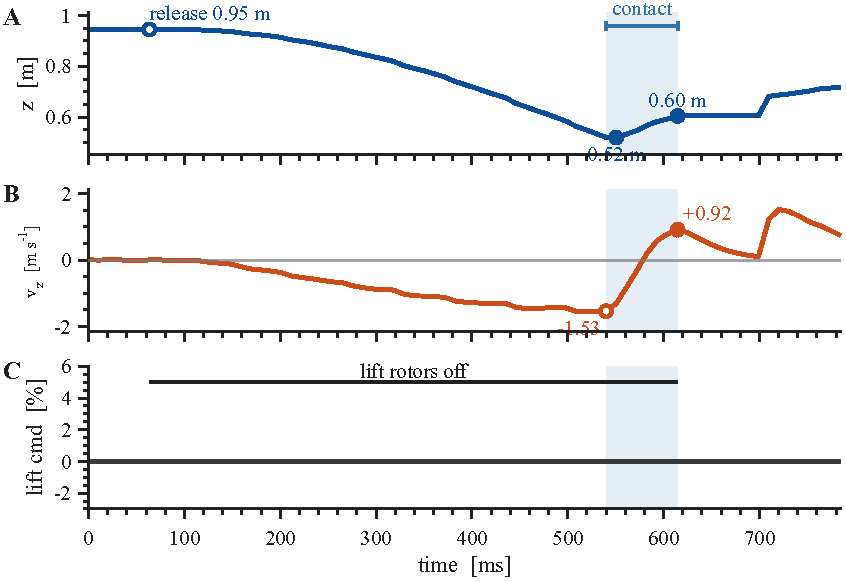
\includegraphics[width=0.72\linewidth]{Assets/ch5fig1_single_hop.pdf}
    \caption{A single water-skipping hop, with the lift rotors commanded
    off throughout.  \textbf{(A)}~Height.  The vehicle is released from a
    hover at $0.94\;\mathrm{m}$, descends to $0.52\;\mathrm{m}$, and has
    recovered to $0.61\;\mathrm{m}$ by the time the foils leave the water.
    \textbf{(B)}~Vertical velocity.  The shaded band marks the water
    contact, bounded by the two turning points of the velocity trace: entry
    at $-1.55\;\mathrm{m\,s^{-1}}$, where the descent stops steepening, and
    exit at $+0.92\;\mathrm{m\,s^{-1}}$, where the water ceases to add
    upward speed.  \textbf{(C)}~Commanded lift thrust, as a percentage of
    full scale.  The command is cut from its hover value to zero before the
    descent and remains there through the contact and ejection; the bar
    marks the unpowered interval.  Control is restored shortly before the
    apex at a thrust-to-weight ratio below $0.35$, which cannot support the
    vehicle and is omitted from the trace for clarity.}
    \label{fig:hop_single}
\end{figure}

%\cleardoublepage
%\include{Chapters/relatedwork}

\cleardoublepage
\chapter{Conclusion and Future Work}
\label{chapter:conclusion}

\section{Summary}

This thesis set out to establish water-skipping as a usable mode of
locomotion for a micro aerial vehicle, and to show that a small rotorcraft can
be thrown back into the air by its own spinning hydrofoils.

The mechanism rests on a single observation: a surface that is nearly useless
in air becomes highly effective the instant it enters water, because the two
fluids differ in density by three orders of magnitude.  A vehicle that spins
continuously can therefore carry hydrofoils at little cost to its flight, and
call on them for a large impulse during a contact lasting only tens of
milliseconds.  Chapter~\ref{dynamic} developed a quasi-steady blade-element
model of that contact, which identifies the inclination of the foils and the
conditions of entry as the quantities that govern the outcome, and shows the
central tension of the manoeuvre: the same sweep that generates the ejecting
force is itself consumed by the water.

Realising this required a vehicle whose spin could be set rather than merely
tolerated.  Chapter~\ref{chapter:paperone} describes an airframe in which two
rotors are mounted tangentially and drive the rotation directly, while two
remain vertical and provide lift and attitude authority.  Decoupling the yaw
drive from the lift channel makes the spin rate an operating parameter chosen
by the experimenter, and, more consequentially for this work, means the
rotation persists when the lift command is removed entirely.  The flight
control that keeps such a vehicle stable and position-controllable while
rotating is developed in Chapter~\ref{chapter:papertwo}, together with the
online separation of the spin-synchronous artefact from the attitude estimate
that makes closed-loop control practical at these rates.

Chapter~\ref{chapter:paperthree} reports the flight experiments.  The vehicle
descends onto the water with its lift rotors commanded to zero, and is
returned to the air by the hydrofoils alone; the controller is re-engaged only
once the vehicle is already climbing away from the surface.  Hops were
repeated, with the vehicle returning to its commanded height between contacts,
demonstrating that the full cycle closes rather than that a single impact can
be survived.

\section{Contributions}

The principal contribution is the locomotion mode itself: a rotorcraft that
travels across water in a sequence of hops, using hydrofoils driven by its own
rotation to recover a substantial part of the energy of each contact.  This
treats the water surface as something to move across rather than as a place to
land, dive, or sample.

Supporting this are a quasi-steady model of hydrofoil-driven ejection that
relates the hop to foil geometry and entry conditions; an airframe whose spin
rate is commanded independently of its lift, which both makes the spin a
design variable and allows the descent to be flown unpowered; and flight
control at spin rates approaching
$10{,}000^{\circ}\,\mathrm{s^{-1}}$, at which no controllability limit was
encountered.

\section{Limitations}

\paragraph{The model over-predicts the contact.}
The blade-element treatment of Chapter~\ref{dynamic} assumes that the foils
are immersed to their geometric depth in an undisturbed, flat surface.  At the
sweep speeds this vehicle reaches, that assumption does not hold: the measured
contact is markedly longer and gentler than predicted, which is consistent
with the free surface deforming away from the foils and with ventilation of
the upper surface.  The model remains useful for the trends it exposes and for
sizing, but its absolute predictions should not be relied upon at these
speeds.

\paragraph{Inertia was never measured.}
The moment of inertia about the spin axis is estimated from a uniform-disk
approximation rather than measured.  Predicted spin loss through the contact
depends on it directly, and should be treated as indicative until it is
determined experimentally.

\paragraph{Instrumentation limited the length of a sequence.}
The number of consecutive hops that could be recorded was limited by the
motion-capture system rather than by the vehicle.  Water thrown up at contact
intermittently interrupts marker tracking at the moment the controller most
needs position feedback.  Mitigations reduced the cost of a dropout to a
single hop, but the limitation is one of the measurement environment, and an
onboard state estimate would remove it.

\section{Future Work}

\paragraph{Contact hydrodynamics.}
The clearest opening is the discrepancy identified above.  Modelling the
deformation of the free surface during entry, rather than assuming it flat,
would close the gap between the predicted and measured contact and turn the
model into a quantitative design tool.  This is also the route to predicting
the depth to which the foils penetrate, which the present treatment cannot.

\paragraph{Disturbed and moving water.}
Every hop reported here was made onto a still surface.  Water encountered
outside a laboratory is not still, and the surface state at the moment of
contact is an untouched variable: waves change the effective entry angle, the
local surface velocity, and the depth available to the foils.  Whether the
vehicle can hop reliably into a disturbed surface, and how the foils should be
shaped if it must, is a natural continuation of this work.

\paragraph{Onboard estimation.}
Removing the dependence on external motion capture would lift the constraint
that limited hop sequences here, and is a precondition for operating outside a
prepared volume.

\paragraph{Phase lag at high spin rate.}
No controllability limit was reached in this work, and the spin rates flown
were well above what earlier reasoning suggested would be workable.  A
plausible explanation is that the binding constraint is the phase lag around
the closed loop rather than the number of control updates per revolution,
since a rotating vehicle turns measurably between a measurement being taken
and the corresponding command taking effect.  This was not investigated: no
latency measurements were recorded, and the observation is offered only as a
direction, not as a result.

\paragraph{Foil design.}
Only one hydrofoil geometry was fabricated and flown.  The inclination and
planform were selected from the model rather than from experiment, and a study
that varies them on hardware would test the model's predictions directly and
is the obvious follow-on to the present work.


\cleardoublepage
\phantomsection
\printbibliography[heading=bibintoc]

\include{Chapters/publications}

\end{document}